\documentclass[a4paper]{scrreprt}
\usepackage{scrextend}
\usepackage[german]{babel}
\usepackage[utf8]{inputenc}
\usepackage[T1]{fontenc}
\usepackage{ae}
\usepackage[bookmarks,bookmarksnumbered]{hyperref}
\usepackage{array}
\newcolumntype{P}[1]{>{\centering\arraybackslash}p{#1}}

%graphics
\usepackage{graphicx}
\graphicspath{ {images/GUI/c-editor/}
 {images/GUI/Eigenschaften-Liste/}
  {images/GUI/Eigenschaften/}
  {images/GUI/Parameter-editor/}
  {images/}} 

\usepackage[printonlyused]{acronym}
\usepackage{hyperref}
\usepackage{float}

%glossary stuff, must be defined after hyperrefs
\usepackage[toc]{glossaries}
\makeglossaries
\newglossaryentry{CBMC}
{
name={C bounded model checker},
description={Ein Programm, welches C-Programme mittels bounded model checking auf Fehler und vom user definierte assertions untersucht}
}
\newglossaryentry{Makro}
{
name={Makro},
description={Ein Codeabschnitt, der durch den Präprozessor ersetzt wird}
}
\newglossaryentry{Benutzer}
{
name={Benutzer},
description={Die Person, welche das Program bedient, Eingaben tätigt, etc}
}

\begin{document}

\title{Pflichtenheft}
\author{Beste Gruppe}
\maketitle 

\tableofcontents	

\listoffigures

\chapter*{Abkürzungsverzeichnis}
\begin{acronym} %put all your abbreviations here 
\acro{CBMC}{C Bounded Model Checker}
\acro{BMC}{Bounded Model Checking}
\acro{GUI}{Graphical User Interface}
\end{acronym}
 
\chapter{Produktübersicht}
Wahlverfahren bilden den Grundstein unserer Demokratie. Dabei werden viele Anforderungen an sie gestellt, welche unsere intuitiven Ideen über Gerechtigkeit formalisieren: Proportionalität, Anonymität, etc. Moderne Wahlverfahren sind oft so komplex, dass sie viele überraschende und teils unerwünschte Eigenschaften haben. Nachweisen deren Abwesenheit ist absolut nicht trivial. So wurde beispielsweise 2008 das Bundestagswahlrecht vom BVerfG für verfassungswidrig erklärt, da es unter anderem die Gleichheit der Wirkung verschiedener Stimmen verletzte. Auf der anderen Seite ist es auch sehr schwer, Wahlverfahren auf die Präsenz erwünschter Eigenschaften zu untersuchen.

\ac{BMC} wird normalerweise dazu verwendet zu überprüfen, ob ein gegebenes Programm gegebene Eigenschaften erfüllt. Da dieses Problem im Allgemeinen unentscheidbar ist, werden nur endliche Codepfade überprüft. Dadurch wird der Zustandsraum endlich und das Problem entscheidbar. Um dies zu bewerkstelligen, werden potentiell unendliche Codepfade - also Schleifen - bis zu einer vom \gls{Benutzer} bestimmten Grenze aufgerollt. Danach wird eine SAT-Formel erstellt, die erfüllbar ist, genau dann wenn das Programm einen Zustand einnehmen kann, welcher die gegebene Eigenschaft nicht erfüllt. Dies ist vollautomatisch und gibt bei Nichterfüllung das Gegenbeispiel zurück.  

In unserem Fall kann \ac{BMC} konkret dazu verwendet werden, ein C-Programm darauf zu untersuchen ob es im Falle gegebener Vorbedingungen gegebene Nachbedingungen erfüllt. Dies wird dazu verwendet, obige Problemstellung innerhalb einer bestimmten Genauigkeit zu lösen: so kann ein in C beschriebenes Wahlverfahren wie z.B. die einfache Mehrheitswahl darauf geprüft werden, ob es bestimmte Eigenschaften erfüllt. Allerdings ist es kompliziert, dies direkt zu tun. 

Unser Programm ist im Wesentlichen eine sehr umfangreiche Schnittstelle um mit \ac{CBMC} zu kommunizieren. Es bietet dem \gls{Benutzer} über eine \ac{GUI} die Möglichkeiten, formale Eigenschaften für Wahlverfahren sowie diese Wahlverfahren selbst anzugeben und zu editieren. Weiterhin liefert es Möglichkeiten, die Interaktion mit \ac{CBMC} zu gestalten: Für wie viele Wähler, Plätze etc die Eigenschaft überprüft werden soll. Nach erfolgreicher Überprüfung durch \ac{CBMC} bekommt der \gls{Benutzer} schließlich eine Antwort des Programms, in der er bei Nichterfüllung der Eigenschaft ein Gegenbeispiel angezeigt bekommt. Wird kein Gegenbeispiel gefunden, so wird eine Erfolgsmeldung ausgegeben. All dies wird graphisch über die \ac{GUI} aufbereitet.

Die \ac{GUI} ist nach Funktionalität in vier Teilen angeordnet:
\begin{enumerate}
\item "`C-Editor"': Code-Editor für Wahlverfahren in der Programmiersprache C
\item "Eigenschaften-Liste": Listenansicht aller Eigenschaften, die für dieses Wahlverfahren untersucht werden sollen
\item "`Eigenschaften-Editor"': Editor für Spezifikation formaler Eigenschaften als boolsche Ausdrücke in eigens dafür vorgesehener Grammatik
\item "`Params"': Eingabe von Parametern einer zu analysierenden Wahl
\end{enumerate}

\section{Die Syntax zur Angabe der formalen Eigenschaften} \label{Sprache-für-formale-Eigenschaften}
In diesem Abschnitt wird ein grober Überblick über die Sprache, welche der Eigenschaften-Editor verwendet, gegeben. Es handelt sich um ein Subset der C-Sprache mit einigen Ergänzungen. Diese werden im Folgenden erläutert. 

Formale Eigenschaften werden in Vor- und Nachbedingungen unterteilt. Diese wiederum werden vom User als eine Liste boolscher Ausdrücke angegeben. Die Sprache erlaubt folgende Konstrukte zur Darstellung boolscher Ausdrücke:

\begin{itemize}
\item Folgende, aus C übernommene binäre Operatoren:
\begin{table}[H]
\begin{tabular}{|p{3cm}|p{1,5cm}|p{4,5cm}|p{3cm}|}
	Operator & Symbol & Erwartet Argumente & Rückgabewert \\
	\hline
	Das logische Und & \verb!&&! & zwei boolsche Ausdrücke & \texttt{true} oder \texttt{false} \\
	Das logische Oder & \verb!||! & zwei boolsche Ausdrücke & \texttt{true} oder \texttt{false}	
	\end{tabular}
\end{table}	

\item Folgende, zusätzlich hinzukommende binäre Operatoren:
\begin{table}[H]
\begin{tabular}{|p{4cm}|p{1,5cm}|p{4,5cm}|p{3cm}|}
	Operator & Symbol & Erwartet Argumente & Rückgabewert \\
	\hline
	Die logische Implikation & \verb!==>! & zwei boolsche Ausdrücke & \texttt{true} oder \texttt{false} \\
	Die logische Äquivalenz & \verb!<==>! & zwei boolsche Ausdrücke & \texttt{true} oder \texttt{false}	
\end{tabular}
\end{table}	

Beispiel: \verb!x > y <==> x + 1 > y + 1! \\
Bedeutung: \verb!x! ist größer als \verb!y! genau dann, wenn auch \verb!x + 1! größer als \verb!y + 1! ist 

\item Folgende, aus C bekannte Operatoren. "'Vergleichbarer Typen"' bedeutet, dass zwei Variablen dieser Typen bereits in C mit demselben Operator vergleichbar sind. 
\begin{table}[H]
\begin{tabular}{|p{2,5cm}|p{1,5cm}|p{6cm}|p{3cm}|}
	Operator & Symbol & Erwartet Argumente & Rückgabewert \\
	\hline
	Gleicheit & \verb!==! & zwei Variablen vergleichbarer Typen & \texttt{true} oder \texttt{false} \\
	Ungleicheit & \verb|!=| & zwei Variablen vergleichbarer Typen & \texttt{true} oder \texttt{false} \\
	kleiner als & \texttt{<} & zwei Variablen vergleichbarer Typen & \texttt{true} oder \texttt{false} \\
	kleiner gleich & \texttt{<=} & zwei Variablen vergleichbarer Typen & \texttt{true} oder \texttt{false} \\
	größer als & \texttt{>} & zwei Variablen vergleichbarer Typen & \texttt{true} oder \texttt{false} \\
	größer gleich & \texttt{>=} & zwei Variablen vergleichbarer Typen & \texttt{true} oder \texttt{false} \\
\end{tabular}
\end{table}	
 	
\item Symbolische Variablen vom Typ Wähler, Kandidat oder Sitz. Für deren Benennung gelten dieselben Regeln wie für die Benennung von Variablen in C. \\

Beispiel: \verb!Wähler v, Kandidat c!

\item Quantoren für Wähler, Kandidaten und Sitze in der Form von \gls{Makro}s. Ein bisher ungenutzter Variablenname wird als Argument erwartet. Dieser kann in dem darauf folgenden Ausdruck als symbolische Variable entsprechenden Typs verwendet werden. \\

Beispiel: \verb|FOR_ALL_VOTERS(v) : EXISTS_ONE_CANDIDATE(c) : v mag c| \\
Bedeutung: Für jeden Wähler (\verb!v!) gibt es zumindest einen Kandidaten (\verb!c!) sodass das Tupel die Eigenschaft "'der Wähler v mag den Kandidaten c"' erfüllt (Dies ist nur ein Beispiel, der Editor wird die Eigenschaft 'mögen' nicht zu Verfügung stellen. An dessen Stelle könnte jedoch jeder andere binäre Operator stehen, welcher eine Variable vom Typ Wähler und eine Variable vom Typ Kandidat erwartet und \texttt{true} oder \texttt{false} zurückgibt).

\item Ausgabe der Anzahl Stimmen für einen Kandidaten in der Form eines Makros.

\item Viele Eigenschaften benötigen zu ihrer Überprüfung das Vergleichen mehrerer Wahldurchläufe. Dies wird ermöglicht durch Variablen VOTESx() und ELECTx. Dabei steht 'x' für die Nummer des Wahldurchangs. VOTESx() erwartet als Argument eine symblische Variable vom Typ Wähler. Zurück gibt es die Stimme, welche v im Wahldurchgang x abgegeben hat. ELECTx erwartet kein Argument und gibt das Wahlergebnis im x-ten Durchgang zurück. Der Rückgabetyp beider Makros hängt von der Kategorie des Wahlverfahrens ab. Gibt das Wahlverfahren zum Beispiel nur einen "'Gewinner"' aus, so ist ELECTx vom Typ Kandidat. \\

Beispiel: \verb|FOR_ALL_VOTERS(v) : VOTES1(v) == VOTES2(v)| \\
Bedeutung: Alle Wähler wählen in beiden Wahlen (\verb!VOTES1! und \verb!VOTES2! ) gleich. \\

Beispiel: \verb|ELECT1 == ELECT2|
Bedeutung: Das Ergebnis des ersten Wahldurchlaufs stimmt mit dem des zweiten Wahldurchlaufs überein.
\item Folgende Konstanten: Anzahl Wähler (\verb!V!), Anzahl Kandidaten (\verb!C!) und Anzahl Sitze. (\verb!S!)
\end{itemize}
Beendet wird ein boolscher Ausdruck durch ein Semikolon. 


\chapter{Zielbestimmung}
Ziel des Programmes ist es eine  Lösung zur Analyse von formalen Eigenschaften von Wahlverfahren zu präsentieren. Die Analyse solcher Eigenschaften ist ein nicht entscheidbares Problem und wird deshalb innerhalb von Grenzen mit Hilfe eine \ac{BMC} ausgeführt. Das Programm soll auch von Nicht-Informatikern mit minimalem Aufwand erlernt und eingesetzt werden können.
Das Programm soll Folgendes bereitstellen:
\begin{itemize}
\item Eine Möglichkeit zur Beschreibung eines Wahlverfahrens, das in C-Code geschrieben ist
\item Eine Möglichkeit zur Beschreibung von formalen Eigenschaften, welche das Wahlverfahren erfüllen soll, in der in \ref{Sprache-für-formale-Eigenschaften} beschriebenen Syntax 
\item Eine Möglichkeit zum Angeben der Parameter des angegebenen Wahlverfahrens (Anzahl Wähler, Anzahl Kandidaten, Anzahl Sitze)
\item Eine Möglichkeit, die Analyse auszuführen
\item Eine Ausgabe des Ergebnisses der Analyse: eine Erfolgsmeldung falls alle Eigenschaften erfüllt werden und Präsentation eines Gegenbeispiels sonst
\end{itemize}

Die Analyse der gegebenen Eigenschaften wird durch \ac{CBMC} geschehen. Aufgabe des Programmes wird es sein, die Eingaben des \gls{Benutzer}s aufzubereiten, so dass \ac{CBMC} aufgerufen werden kann. Die Ausgabe von \ac{CBMC} wird dann vom Programm interpretiert und dem Benutzer präsentiert. 

Die Analyse der Eigenschaften lässt sich auch schon ohne Verwendung unseres Programms erledigen. Allerdings wäre der damit verbundene Lern- und Einarbeitungsaufwand sehr hoch, vor allem bei der Eingabe formaler Eigenschaften. Weiterhin ist damit viel, sich jedes Mal wiederholender Aufwand, verbunden, der sich automatisieren lässt. Daher ist ein Schwerpunkt unseres Programms einfache Benutzbarkeit, besonders für Nicht-Informatiker. Dies soll erreicht werden über eine \ac{GUI}, welche oft benötigte Funktionalität bereitstellt. Einfache syntaktische Fehler im Code sollen während des Editierens erkannt werden. Dadurch soll das Untersuchen von Wahlverfahren leichter und schneller werden, was den Mehrwert unseres Programmes ausmacht.

\section{Musskriterien}
\subsection{Allgemein}
\begin{itemize}
\item Das Programm kann auf 32-Bit Versionen von Windows und Linux-Betriebssystemen betrieben werden
\item Alle Abhängigkeiten werden mit dem Programm ausgeliefert
\end{itemize}

\subsection{C-Editor}
Das Programm bietet einen Editor für das zu prüfende Wahlverfahren. Der Editor erwartet eine Eingabe in der Programmiersprache C.\\
Folgende Funktionalität bietet der C-Editor:
\begin{itemize}
	\item Eingegebener Code kann abgespeichert werden
	\item Gespeicherter Code kann in den C-Editor geladen werden
	\item Der Code-Editor zeigt Fehler im eingegebenen Code an
	\item Aktionen können widerrufen und wiederhergestellt werden
\end{itemize}
	
\subsection{Eigenschafteneditor}
Es können formale Eigenschaften eingegeben werden. Die Eingabe erfolgt in der in \ref{Sprache-für-formale-Eigenschaften} beschriebenen Syntax. Die eingegebenen Eigenschaften sind Parameter bei der Ansteuerung von \ac{CBMC}.\\
Folgende Funktionalität bietet der Eigenschafteneditor:
\begin{itemize}
	\item Eine formale Eigenschaft kann abgespeichert werden
	\item Gespeicherte Eigenschaften können in den Eigenschafteneditor geladen werden	
	\item Fehler in der Eingabe werden angezeigt
\end{itemize}

\subsection{Parametereditor}
Parameter für eine Wahl (Anzahl der Wähler, Kandidaten und Sitzen) können festgelegt werden. Bei der Analyse wird das Wahlverfahren nur innerhalb dieser Wahlparameter geprüft. Werden keine Parameter angegeben, wird \ac{CBMC} ohne sie aufgerufen.\\
Folgende Funktionalität bietet der Parametereditor:
\begin{itemize}
	\item Die Anzahl der Wähler kann festgelegt werden
	\item Die Anzahl der Kandidaten kann festgelegt werden
	\item Die Anzahl der Sitze kann festgelegt werden
	\item Die Analyse des Wahlverfahrens kann gestartet werden
	\item Es kann ein Timeout festgelegt werden, nach dem die Analyse automatisch abgebrochen wird
\end{itemize}

\subsection{Eigenschaftenliste}
Das Ergebnis der Analyse wird vom Programm graphisch ausgegeben. 
\begin{itemize}
	\item Falls alle Eigenschaften erfüllt sind, wird eine Erfolgsmeldung ausgegeben
	\item Ansonsten wird ein Gegenbeispiel ausgegeben
\end{itemize}


\section{Sollkriterien}
\subsection{C-Editor}
Folgende Funktionalität bietet der C-Editor zusätzlich:
\begin{itemize}
	\item Syntax-Highlighting
	\item Automatisches Einrücken
	\item Tastatur-Shortcuts
	\item Codevorlagen können in den Editor geladen werden
\end{itemize}

\subsection{Eigenschafteneditor}
Folgende Funktionalität bietet der Eigenschafteneditor zusätzlich:
\begin{itemize}
	\item Code completion
\end{itemize}

\subsection{Parametereditor}
Folgende Funktionalität bietet der Parametereditor zusätzlich:
\begin{itemize}
	\item Die Anzahl der Wähler kann als Intervall festgelegt werden (von x bis y Wähler, x < y)
	\item Die Anzahl der Kandidaten kann als Intervall festgelegt werden (von w bis z Kandidaten, w < z)
	\item Die Anzahl der Sitze kann als Intervall festgelegt werden (von m bis n Sitzen, m < n)
	\item Die Analyse von \ac{CBMC} kann jederzeit abgebrochen werden
\end{itemize}

\subsection{Eigenschaftenliste}
Vordefinierte Standardeigenschaften (z.B. Anonymität) können einzeln in die Analyse mitaufgenommen werden. \\
Das Ergebnis der Analyse für diese Standardeigenschaften wird für jede Eigenschaft einzeln ausgegeben.


\section{Wunschkriterien}
\subsection{Allgemein}
\begin{itemize}
\item Das Programm kann auf einem Mac betrieben werden
\end{itemize}

\subsection{C-Editor}
Folgende Funktionalität bietet der C-Editor zusätzlich:
\begin{itemize}
	\item Warnung vor nicht unterstützten Elementen der Programmiersprache wie z.B. Threads
\end{itemize}

\subsection{Parametereditor}
Es kann eine Wahl als Stimmenarray eingegeben werden. Das Ergebnis der Wahl wird in der Eigenschaftenliste angezeigt.


\section{Abgrenzungskriterien}
\begin{itemize}
\item Das Programm kann keine Angabe darüber machen, wie lange die Überprüfung einer Eigenschaft dauern wird
\end{itemize}



\chapter{Produkteinsatz}
Das Programm dient dazu, Wahlverfahren auf ihre formalen Eigenschaften hin zu analysieren. Es richtet sich an Benutzer, die ein Interesse an der Erforschung oder Entwicklung solcher Wahlverfahren haben. Diese Benutzer werden hauptsächlich aus dem Bereich der theoretischen Informatik oder der Politwissenschaft stammen. Deshalb soll das Programm auch für Nicht-Informatiker zugänglich sein. Für die Bedienung des Programms ist jedoch Kenntnis der Programmiersprache C und der Aussagen- und Prädikatenlogik nötig.\\
Das Erstellen von neuen Wahlverfahren gestaltet sich ohne Hilfsmittel als schwierig. Besonders aber die Analyse solcher Wahlverfahren auf die Einhaltung von gegebenen Vor- und Nachbedingungen ist für viele Menschen eine Unmöglichkeit. Das Produkt soll diese Analyse stark vereinfachen.\\

\section{Anwendungsbereiche}
\begin{itemize}
\item Universität
\item Forschung
\end{itemize}

\section{Zielgruppen}
\begin{itemize}
\item Wahlforscher
\item Softwareentwickler
\item Hobbyisten
\end{itemize}

\section{Betriebsbedingungen}
\begin{itemize}
\item Das Produkt kommt in einer Büroumgebung zum Einsatz. Es wird auf einem
aktuellen Computer mit entsprechenden Werten für Arbeitsspeicher und Rechnergeschwindigkeit betrieben.
\end{itemize}

\section{Szenarien}
\textbf{Szenario 1}\\
Ein Wahlforscher wird von der Regierung eines Landes beauftragt ein neues Wahlverfahren zu entwerfen. Dieses soll bestimmte, vorgegebene formale Eigenschaften erfüllen.\\
Er installiert das Tool und entwickelt mit diesem eine erste Version des Wahlverfahrens. Zusätzlich gibt er die vorgegebenen Eigenschaften als formale Eigenschaften in das Tool ein.\\
Nun gibt er Parameter zum Prüfen an (Wähler, Stimmen, Sitze) und lässt das Wahlverfahren auf die formalen Eigenschaften prüfen.\\
Das Tool gibt aus, dass nicht alle Eigenschaften vom Wahlverfahren erfüllt werden.\\
Mithilfe der Informationen aus der Ergebnisausgabe analysiert und modifiziert der Entwickler das Wahlverfahren so, dass es alle Eigenschaften erfüllt.\\
Er prüft es nochmals auf alle Eigenschaften und nun werden alle erfüllt.\\
Zuletzt speichert er Wahlverfahren und formale Eigenschaften ab und sendet ersteres an eine Prüfstelle für Wahlverfahren.

\begin{figure}[H]
\hspace{-1cm}
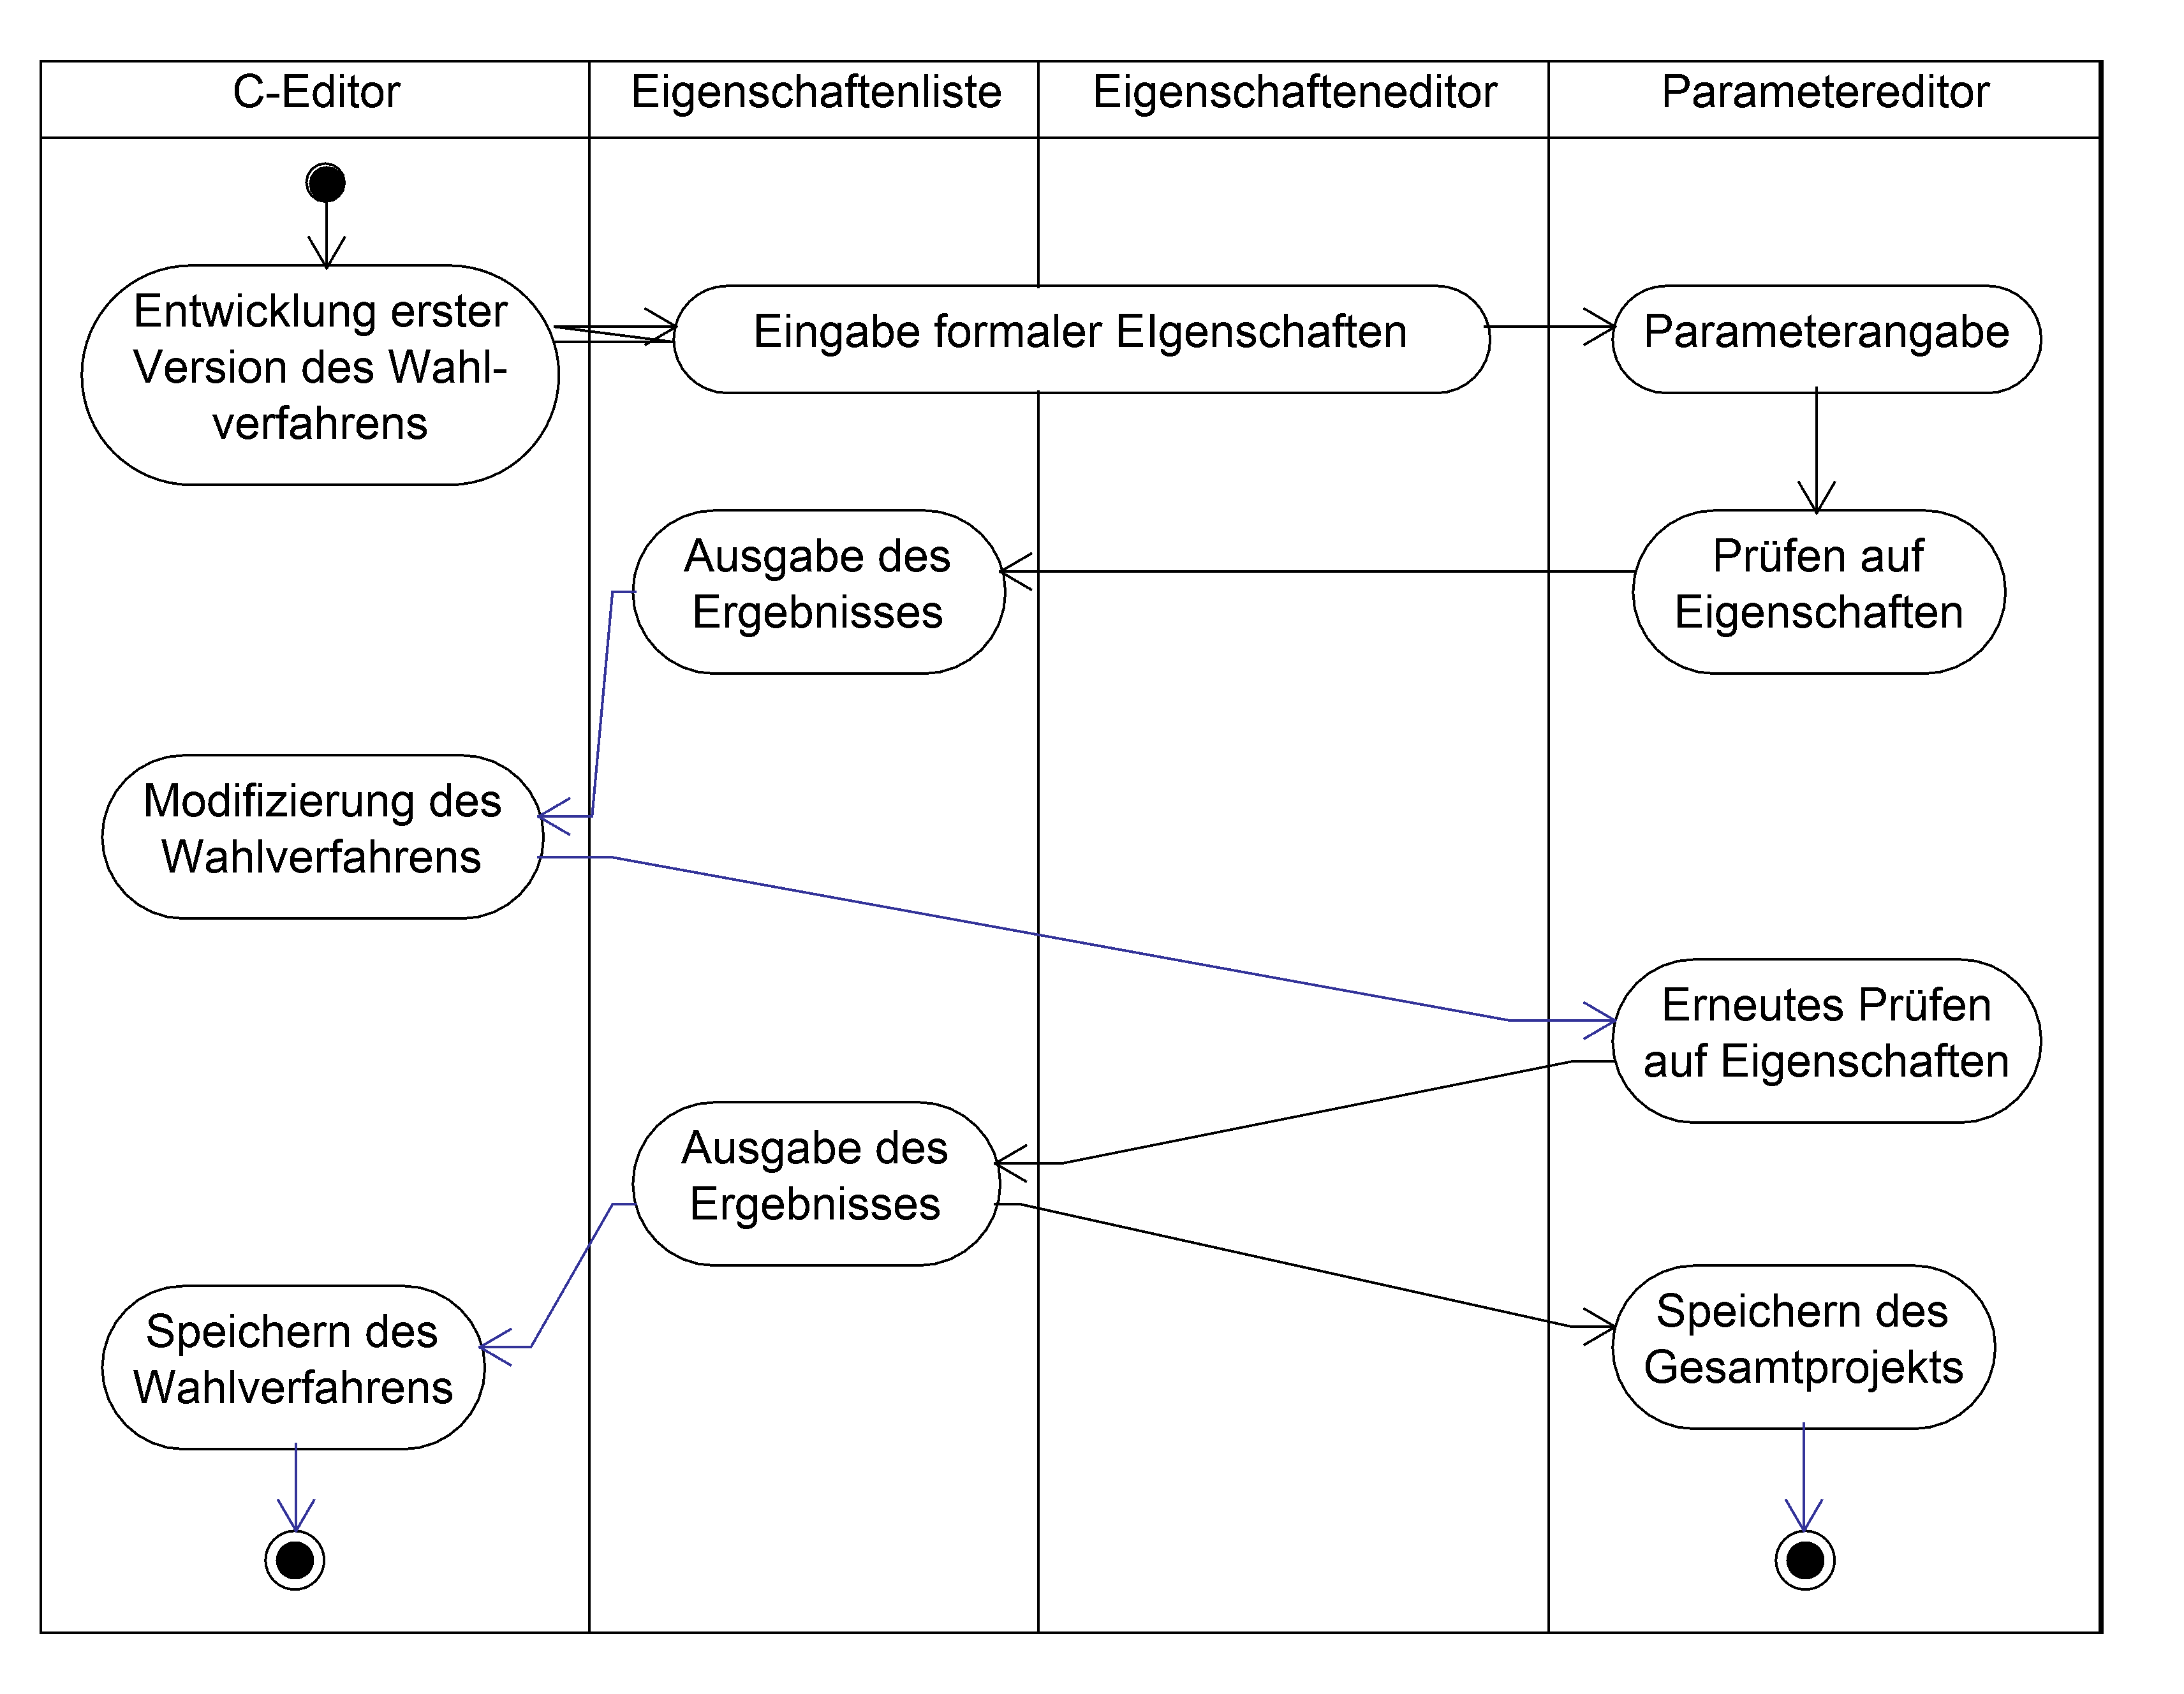
\includegraphics[scale=0.12]{ActivityDiagramScenario1.png}
\caption{Aktivitätsdiagramm zu Szenario 1}
\label{Packet-scetch}
\end{figure}

\textbf{Szenario 2}\\
Eine Prüfstelle bekommt ein Wahlverfahren übergeben welches sie auf bestimmte formale Eigenschaften testen soll.\\
Das Tool wird installiert und das Wahlverfahren im C-Editor geladen und es werden formale Eigenschaften erstellt.\\
Um das Wahlverfahren auf die Eigenschaften zu prüfen werden Parameter zu \\Kandidaten-, Stimmen- und Wähleranzahl, sowie einem Timeout als obere Zeitgrenze für das Prüfen angegeben.\\
Wenn das Tool fertig mit dem Überprüfen ist, werden erfüllte und nichterfüllte Eigenschaften angezeigt. Diese Informationen benutzt die Prüfstelle dann in ihrem Bericht über das Wahlverfahren.\\

\begin{figure}[H]
\hspace{-1cm}
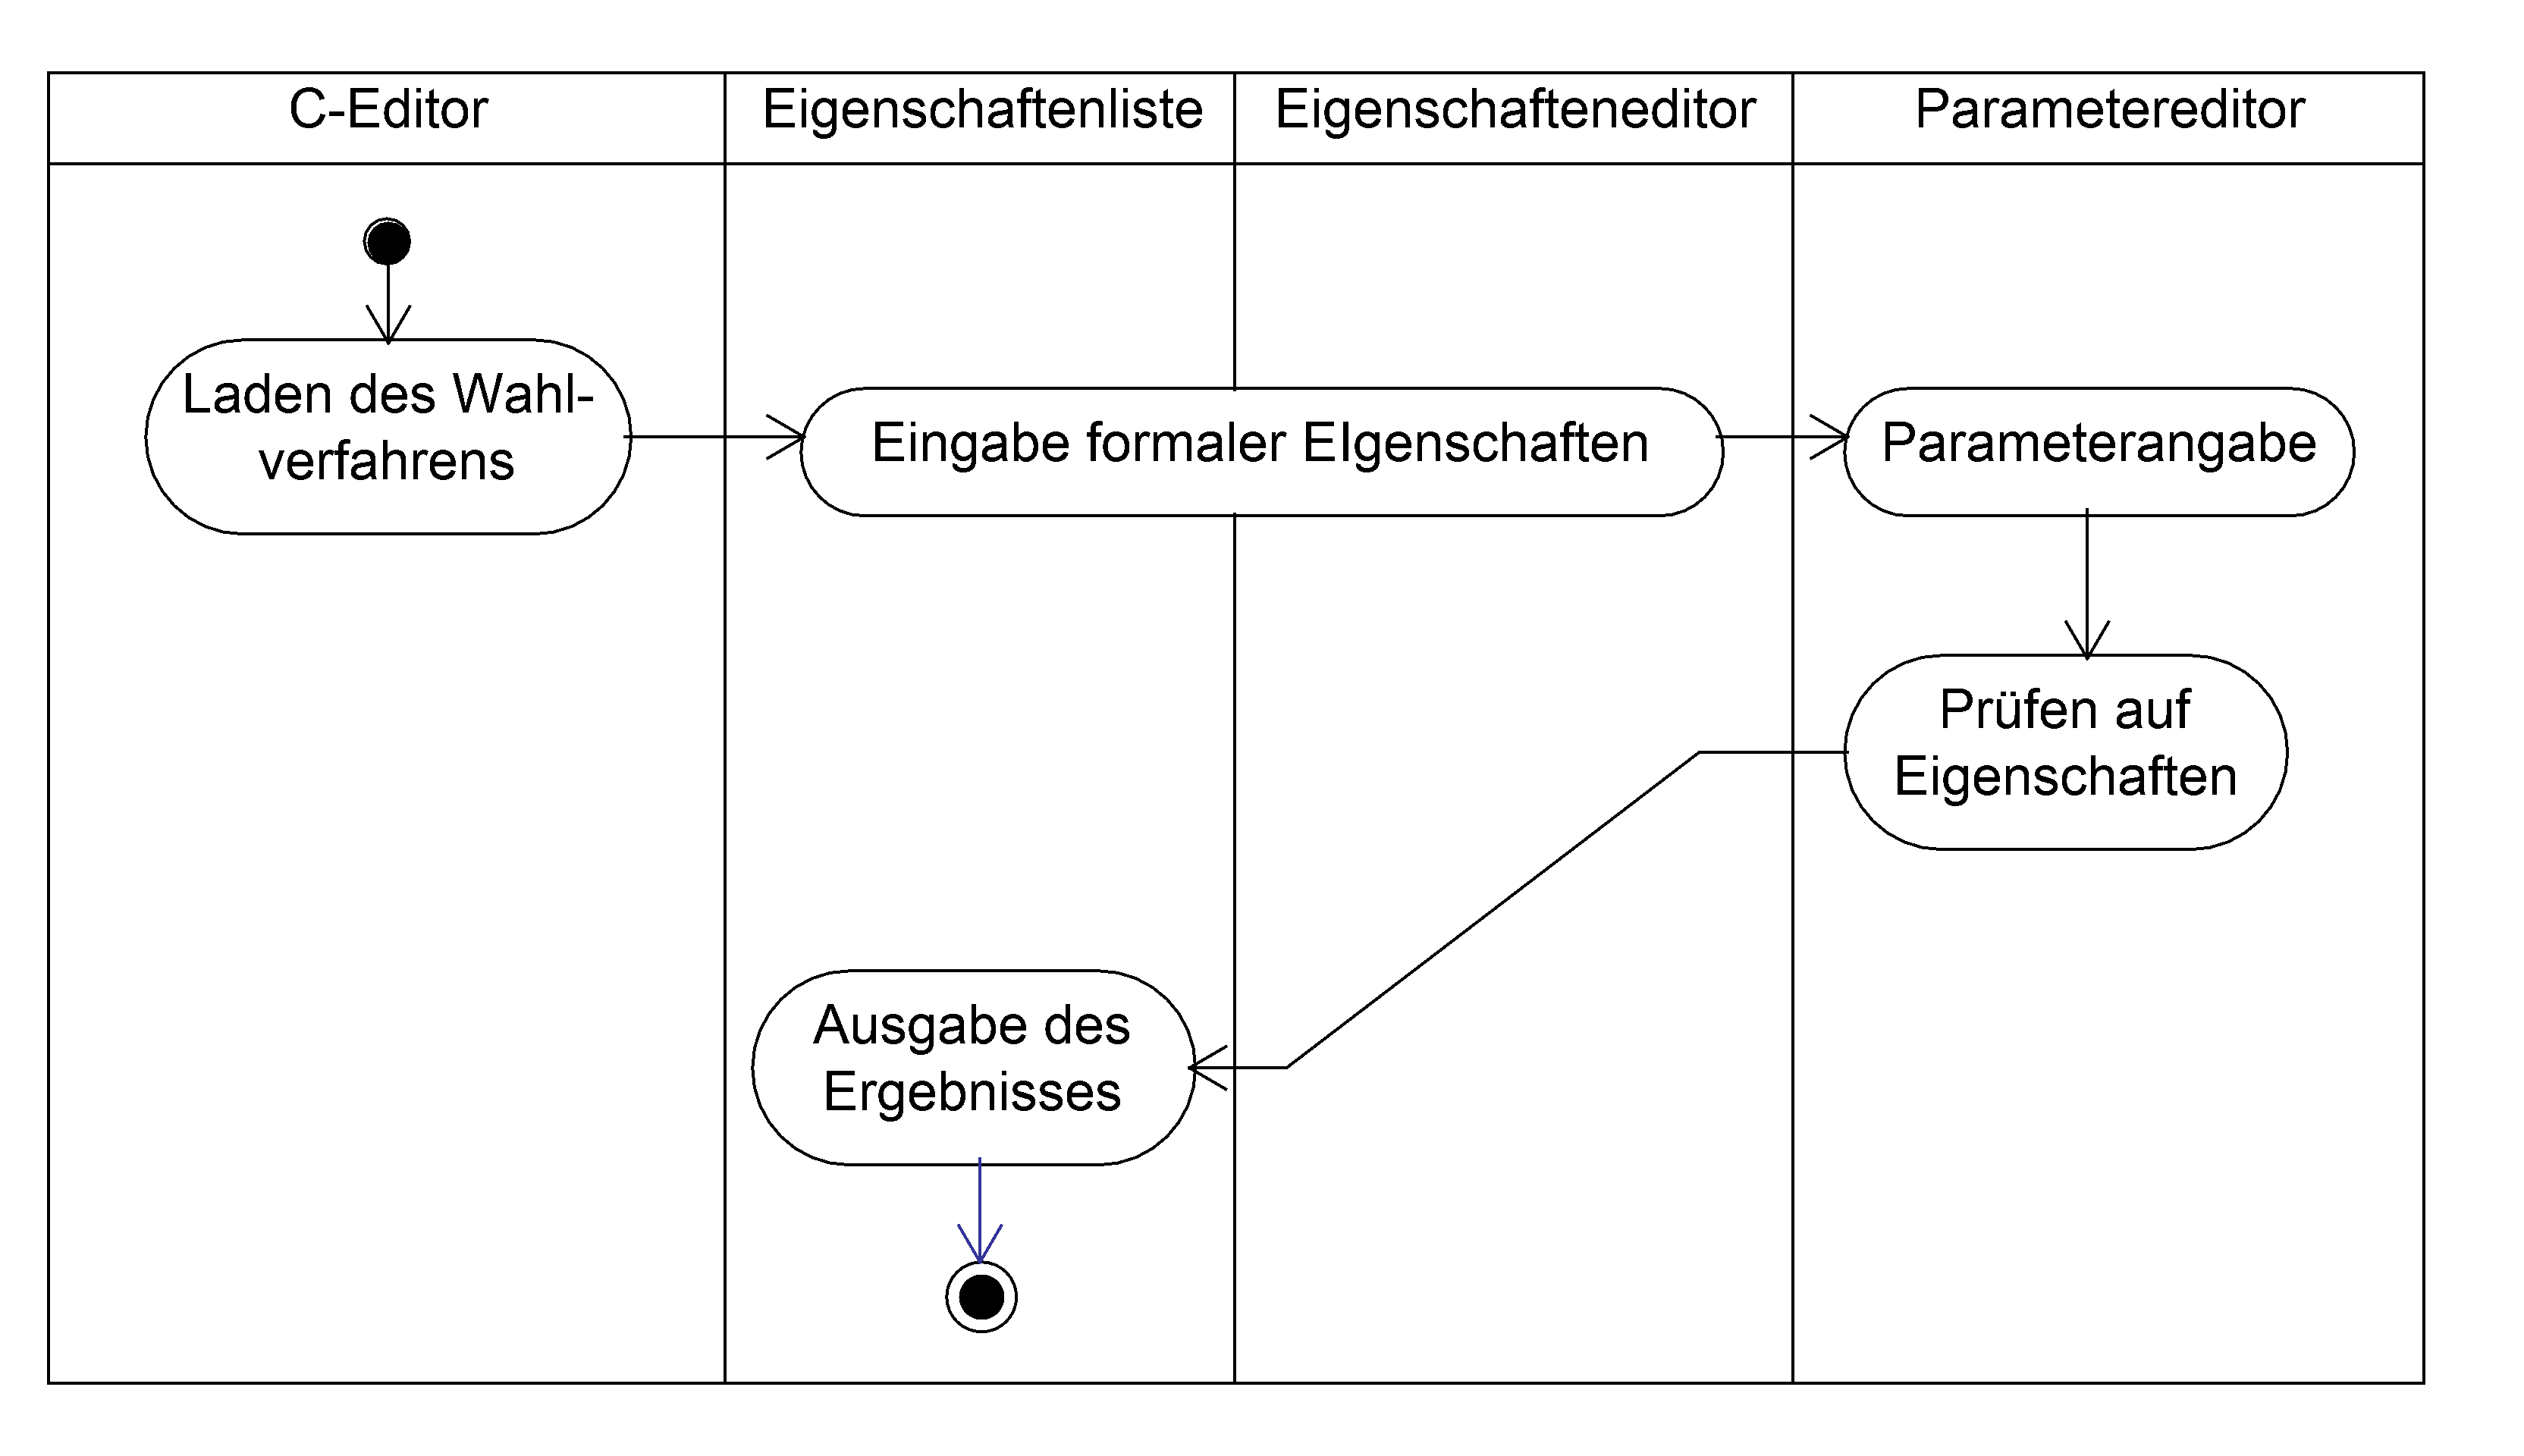
\includegraphics[scale=0.12]{ActivityDiagramScenario2.png}
\caption{Aktivitätsdiagramm zu Szenario 2}
\label{Packet-scetch}
\end{figure}

\chapter{Produktumgebung}

\section{Software}
\begin{itemize}
\item Das Betriebssystem ist entweder Microsoft Windows (7,8 oder 10) oder eine der Linux-Distributionen Arch oder Ubuntu.
\item Java SE Runtime Environment 8 ist installiert.
\item Ist das Betriebssystem Microsoft Windows 7, 8 oder 10 benötigt man zusätzlich
\begin{itemize}
\item Die Developer Command Prompt für Visual Studio
\item cl.exe, ein tool welches die Microsoft Compiler und Linker kontrolliert. Es wird ebenfalls mit Visual Studio geliefert.
\end{itemize}
\end{itemize}

\section{Hardware}
\begin{itemize}
\item Arbeitsspeicher: 4 GB DDR3 RAM oder besser
\item Prozessor: Intel i3 dual core mit 2 * 1,7 GHz oder äquivalent
\item Grafik: Intel HD3000 oder besser
\item Maus, Tastatur und Bildschirm
\end{itemize}

\section{Produkt-Schnittstellen}
\begin{itemize}
\item ANTLR zur Echtzeit-Überprüfung des Codes
\item CBMC zur Überprüfung der formalen Eigenschaften
\item GNU C-Compiler zur statischen Analyse des C-Codes
\end{itemize}

\chapter{Funktionale Anforderungen}
\section{Allgemein}
\subsection{Muss-Kriterien}
/FM0010/ Bereitstellen von Editoren zur Beschreibung des Wahlverfahrens sowie zur Beschreibung zu erfüllender formaler Eigenschaften \\
/F0020/ Kommunikation und Überprüfung dieser Eigenschaften via \ac{CBMC} \\
/FM0030/ Bereitstellen von Kommunikationsschnittstellen mit \ac{CBMC} sowohl für Eingabe von Parametern als auch zur Ausgabe der Ergebnisse einer Überprüfung \\
/FM0031/ Darstellung der Ergebnisse einer Überprüfung in für Nicht-Informatiker verständlicher Form:
\begin{itemize}
\item Zahlen in Dezimaldarstellung
\item Ausgabe der Eingabeparameter des Wahldurchlaufs bzw. der Wahldurchläufe:
\begin{itemize}
\item Ausgabe des Stimmen Arrays (Anzahl Stimmen und Stimmen) 
\item Ausgabe der Kandidaten (Anzahl)
\item Ausgabe der Sitze (Anzahl)
\end{itemize}
\item Ausgabe des Ergebnisses des Wahldurchlaufs bzw. der Wahldurchläufe
\end{itemize} 
/FM0040/ Möglichkeit des Speicherns von Code, formaler Anforderungen und Eingabeparametern als ein Projekt \\
/FM0050/ Möglichkeit des Öffnens und Editierens der Projekte aus /F0040/


\section{C-Code Editor für Wahlverfahren}
\subsection{Muss-Kriterien}
/FM1010/ Darstellung aller für das Programmieren in C benötigten Zeichen \\
/FM1020/ Veränderung des dargestellten Textes durch Eingabe über Tastatur und Maus wie in Notepad \\
/FM1030/ Speichern von erstelltem Code als Datei auf der Festplatte an vom User angegebenen Ort \\
/FM1040/ Laden und Darstellen von Dateien korrekten Formats \\
/FM1050/ Anzeigen syntaktischer Fehler in dem Fehler Fenster (siehe \ref{Editor-mit-Fehler-nach-statischer-analyse}). Nicht asynchron während Eingeben des Codes sondern synchron nach Eingabe des entsprechenden Befehls.

\subsection{Soll-Kriterien}
/FS1060/ Überprüfen des Formats beim Ladevorgang. Falls falsches Format: Ausgabe einer Fehlermeldung \\
/FS1070/ Syntax-Highlighting: Darstellung diverser Schlüsselwörter in anderen Farben als den Rest des Codes. Dies beinhaltet, ist jedoch nicht beschränkt auf: 
\begin{itemize}
\item Typendeklaration (int, float, ...)
\item Kontrollflow-Konstrukte (if, else, while...)
\item Variablennamen
\item Kommentare
\end{itemize}
/FS1080/ Anzeigen der Zeilennummern am linken Zeilenrand \\
/FS1090/ Anzeigen von Syntaktischen Fehlern im Code, welche durch einen Lexer oder Parser erkannt werden können: 
\begin{itemize}
\item Verwendung von Schlüsselwörtern als Variablennamen 
\item Vergessene Semikolons am Ende von Anweisungen
\item Nicht geschlossene Klammern und Anführungszeichen
\item Andere Konstrukte, welche der Grammatik der C-Sprache widersprechen
\end{itemize}
Wie /FM1050/ ist dies von /FK1150/ abgegrenzt durch synchronen Aufruf der Funktionalität.

Reaktion auf typische Tastenkürzel\\
\begin{table}[H]
\caption{Hotkeys und verbundene Operationen}
\begin{tabular}{lcr} 
Kürzel & Operation \\
\hline 
Strg + c & Kopieren \\
Strg + x & Auschneiden \\
Strg + v & Einfügen \\
Strg + z & Zuletzt ausgeführte Aktion Rückgängig machen \\
Strg + r & Zuletzt rückgängig gemachte Aktion erneut ausführen \\
Strg + s & Speichern \\
Strg + o & Öffnen \\
Strg + Leer & Anzeigen der Code-Completion Vorschläge\\
\end{tabular}
\label{table:Hotkeys_and_operations}
\end{table}

/FS1110/ Bereitstellen von Wahl-Templates
\begin{itemize}
\item Jeder Wähler wählt genau einen Kandidaten
\item Jeder Wähler ordnet Kandidaten nach Präferenz in absteigender Reihenfolge 
\item Jeder Wähler ordnet Kandidaten eine Nummer zwischen MAX (maximale Zustimmung) und MIN (maximale Abneigung) zu. MAX und MIN sind dabei vom User konfigurierbar. 
\item Jeder Wähler gibt zu jedem Kandidaten entweder ein Ja oder Nein ab. Zustimmungswahl.
\end{itemize}

\subsection{Kann-Kriterien}
/FK1120/ Automatisches Einrücken des Codes in Schleifen und if-Statements \\
/FK1130/ Code-Completion
\begin{itemize}
\item Automatisches Schließen von Klammern und Anführungszeichen
\item Primitiv: Vorschlagen bereits im Code vorgekommener Wörter
\item Intelligent: Durch Analysieren eines ASTs nur Vorschlagen der Wörter welche im Kontext Sinn ergeben.
\end{itemize}

/FK1140/ Durch den User konfigurierbares Verhalten:
\begin{itemize}
\item Festlegen der Farben, welche beim Syntax-Highlighting verwendet werden
\item Festlegen des verwendeten Fonts
\item An- und Ausschalten der angezeigten Zeilennummern
\item Festlegen wie vielen Leerzeichen ein Tab entspricht
\end{itemize}
/FK1150/ Anzeige syntaktischer Fehler im Code Editor asynchron während Eingabe des Codes.
 
\section{Editor für formale Eigenschaften}
\subsection{Muss-Kriterien}
/FM2010/ Darstellung aller für das Programmieren in C benötigten Zeichen \\
/FM2020/ Veränderung des dargestellten Textes durch Eingabe über Tastatur und Maus wie in Notepad \\
/FM2030/ Beschreibung von formalen Eigenschaften als Vor- und Nachbedingung  \\
/FM2040/ Beschreibung der Vor- und Nachbedingungen als Auflistung boolscher Ausdrücke (siehe \ref{Sprache-für-formale-Eigenschaften})\\
/FM2050/ Bereitstellung von Makros zur Beschreibung der Eigenschaften (siehe \ref{table:Macros_for_formal_Attributes}) \\

\begin{table}[H]
\caption{Makros zur Beschreibung formaler Eigenschaften}
\begin{tabular}{|p{5cm}|p{10cm}|}
\hline 
Makro & Effekt \\
\hline 
\verb!FOR_ALL_VOTERS(i)! & In der darauf folgenden Eigenschaft kann i als symbolische Variable verwendet werden. Gesamtausdruck ist wahr falls sie für alle Wähler gilt \\
\hline 
\verb!FOR_ALL_CANDIDATES(i)! & In der darauf folgenden Eigenschaft kann i als symbolische Variable verwendet werden. Gesamtausdruck ist wahr falls sie für alle Kandidaten gilt \\
\hline 
\verb!FOR_ALL_SEATS(i)! & In der darauf folgenden Eigenschaft kann i als symbolische Variable verwendet werden. Gesamtausdruck ist wahr falls sie für alle Sitze gilt \\
\hline 
\verb!EXISTS_ONE_VOTER(i)! & In der darauf folgenden Eigenschaft kann i als symbolische Variable verwendet werden. Gesamtausdruck ist wahr falls sie für mindesten einen Wähler gilt \\
\hline 
\verb!EXISTS_ONE_CANDIDATE(i)! & In der darauf folgenden Eigenschaft kann i als symbolische Variable verwendet werden. Gesamtausdruck ist wahr falls sie für mindesten einen Kandidaten gilt \\
\hline 
\verb!EXISTS_ONE_SEAT(i)! & In der darauf folgenden Eigenschaft kann i als symbolische Variable verwendet werden.Gesamtausdruck ist wahr falls sie für mindesten einen Sitz gilt \\
\hline 
\verb!VOTE_SUM_FOR_CANDIDATE(c)! & Gibt die Anzahl Stimmen für Kandidaten c zurück\\
\hline 
\end{tabular}
\label{table:Macros_for_formal_Attributes}
\end{table}

/FM2060/ Bereitstellen symbolischer Variablen für Wähler, Kandidaten und Sitze \\
/FM2070/ Bereitstellen von Operatoren für Implikation und Äquivalenz \\
/FM2071/ Bereitstellen von Operatoren für logisches UND, ODER, GLEICH und NICHT GLEICH \\
/FM2072/ Bereitstellen von Vergleichen: Kleiner, Kleiner gleich, größer, größer gleich,  Gleicheit und Ungleicheit zwischen Typen die diese Vergleiche auch in C zulassen \\
/FM2073/ Möglichkeit zur Abfrage der Stimme eines Wählers v in Wahldurchlauf Nummer x durch VOTESx(v)\\
/FM2080/ Möglichkeit zur Abfrage des Ergebnisses von Wahldurchlauf Nummer x durch ELECTx \\
/FM2090/ Beliebig tiefe, lediglich von Hardware begrenzte, Schachtelung dieser Konstrukte \\
/FM2100/ Möglichkeit zum Speichern von Eigenschaften \\
/FM2110/ Möglichkeit zum Laden und Bearbeiten von Eigenschaften in korrektem Format \\
/FM2120/ Sanity-Checks: Nur korrekte boolsche Ausdrücke werden zugelassen.

\subsection{Soll-Kriterien}
/FS2120/ Syntax-Highlighting \\
/FS2130/ Anzeigen von Syntaktischen Fehlern im Code \\
/FS2131/ Reaktion auf typische Tastenkürzel wie in /FS1100/, siehe \ref{table:Hotkeys_and_operations}. \\


\subsection{Kann-Kriterien}
/FK2140/ Code-Completion
\begin{itemize}
\item Auto-Vervollständigung der Makros
\item Analyse des Codes und Anzeigen relevanter, bereits definierter Eigenschaften und symbolischer Variablen
\end{itemize}

\section{Eigenschaften-Liste}
\subsection{Muss-Kriterien}
/FM3010/ Darstellung der zu analysierenden Eigenschaften in Listenform \\
/FM3020/ Möglichkeit zum Erstellen neuer Eigenschaften \\
/FM3030/ Möglichkeit zum Hinzufügen bereits vorhandener Eigenschaften \\
/FM3040/ Möglichkeit zum Entfernen von Eigenschaften \\
/FM3050/ Möglichkeit das Überprüfen einzelner Eigenschaften an- und auszustellen \\
/FM3060/ Möglichkeit Listen zu Speichern \\
/FM3070/ Möglichkeit Listen in korrektem Format zu Laden \\


\section{Editor für Eingabeparameter}
\subsection{Muss-Kriterien}
/MF4010/ Möglichkeit zur Angabe der zu analysierenden Anzahl von Wählern, Kandidaten und Sitzen \\
/MF4011/ Möglichkeit die Parameter in /F4010/ als Minimum und Maximum anzugeben, welche nacheinander abgearbeitet werden \\
/FM4020/ Sanity-checks der eingegebenen Parameter: Alle größer 0, Minimum kleiner gleich Maximum \\
/FM4030/ Möglichkeit zum Eingeben einer Zeitspanne nach welcher die Berechnung abgebrochen wird \\
/FM4040/ Möglichkeit direkter Eingabe von Argumenten, welche dem Aufruf von CBMC mitgegeben werden \\
/FM4050/ Möglichkeiten das momentan geöffnete Wahlverfahren, die momentan eingestellten Parameter und die momentan geöffnete Eigenschaften-Liste als Projekt zu speichern \\
/FM4060/ Möglichkeit die Projekte aus /F4050/ zu öffnen und zu bearbeiten
/FM4070/ Möglichkeit Überprüfungen zu starten
/FM4070/ Möglichkeit Überprüfungen zu beenden

\chapter{Produktdaten}
\section{Code-Editor Wahlverfahren}
/D10/ Das Wahlverfahren wird vom \gls{Benutzer} als C-Code definiert und in einer Datei mit vom \gls{Benutzer} gegebenen Namen und der Endung .c gespeichert.
/D11/ Die verfügbaren Kategorien an Wahlverfahren werden in einer Datei namens electionTemplates gespeichert.

\section{Editor von formalen Eigenschaften}
/D20/ Eine vom \gls{Benutzer} dafinierte formale Eigenschaft wird in einer Datei mit vom \gls{Benutzer} gegebenen Namen und der Endung .eig gespeichert.

\section{Parameter}
/D30/ Angegebene Parameter für Wahlen werden in einer Textdatei gespeichert.


\section{Projektdaten}
/D40/ Ein Projekt wird als Liste von Dateien in einer Textdatei gespeichert.

\section{Eigenschaften-Liste}
/D50/ Die in der Eigenschaften-Liste erstellten Listen werden in Textdateien gespeichert

\chapter{Nichtfunktionale Anforderungen}
/NF10/ Nicht mehr als 0,5 Sekunden Verzögerung bei Erfragen der Code-Completion \\
/NF20/ Maximal 10000 Kandidaten, Wähler oder Sitze pro Überprüfung \\
/NF30/ Maximal 10000 Zeilen C-Code \\
/NF40/ Maximal 100 Vor- und Nachbedingungen pro formaler Eigenschaft \\
/NF50/ Maximal 50 symbolische Variablen pro formaler Eigenschaften \\
/NF60/ Maximal 10 Jahre währender timeout \\


\chapter{Globale Testfälle und Testszenarien}

Generell testet ein Testfall nicht alle Funktionen einer aufgelisteten funktionalen Eigenschaft. Somit müssen alle Tests, in denen eine funktionale Eigenschaft aufgelistet ist, gelingen, damit eine funktionale Eigenschaft als erfüllt gilt. \\
Innerhalb des kompletten Kapitels 8 ist mit dem Ausdruck \textbf{Dokument} je nachdem welches GUI-Fenster betrachtet wird etwas anderes gemeint. Außerdem werden Im Text GUI-spezifische Sonderfälle mit einem Kürzel markiert. \\
Im Falle des \textbf{C-Editors} handelt es sich um den C-Code und das Kürzel \textbf{C}. \\
Im Falle des \textbf{Eingeschafteneditors} handelt es sich um eine spezifische Eigenschaft von Wahlverfahren und das Kürzel \textbf{E}. \\
Im Falle der \textbf{Eigenschaftenliste} handelt es sich um die Liste der Eigenschaften von Wahlverfahren und das Kürzel \textbf{L}. \\
Im Falle des \textbf{Parametereditors} handelt es sich um den kompletten Programmzustand. Genauer gesagt also den C-Code, die Parameter und die Eigenschaften für Wahlverfahren inklusive der kompletten Eigenschaften-Liste. Der Kürzel für den Parametereditor lautet \textbf{P}. \\ \\

\section{Testfälle für die Datenverwaltung}

Die Testfälle innerhalb dieses Abschnittes betreffen alle 4 GUI-Elemente. \\\\
\textbf{/T010/}\\
\textbf{Prozess: }Erstellen eines neuen Dokuments  \\
\textbf{Abgedeckte Funktionale Anforderungen:} \\
C: /FS1030/ /FS1100/ /FS1110/ \\
E: /FM2100/	\\
L: /F3020/ \\
P: /F4050/	\\
\textbf{Ziel:} Es kann ein neues Dokument angelegt werden\\
\textbf{Kategorie:} muss\\
\textbf{Vorbedingung:} Das Programm wartet auf eine Eingabe. Der Benutzer wählt einen korrekter Speicherpunkt und einen gültiger Dateiname.\\
\textbf{Nachbedingung (Erfolg):} Das Programm zeigt ein neues, leeres Dokument an, das einen Speicherplatz und einen Namen hat.\\
C: Die für das gewählte Wahl-Template benötigten Funktionsrümpfe werden generiert.
\textbf{Nachbedingung (Fehlschlag):} Es wurde kein neues, leeres Dokument angelegt und dargestellt\\
\textbf{Akteur:} Benutzer\\
\textbf{Auslösendes Ereignis:} Der Benutzer will ein neues Dokument anlegen\\
\textbf{Beschreibung:} \\
1. C: Der Nutzer drückt Strg + N \\
Allgemein (auch für C gültig): Der User betätigt den Button Neu des jeweiligen Fensters. \\
2. Das Programm öffnet einen Dateibrowser.\\
3. Der User gibt den Speicherort und den Name des neuangelegten Dokuments an. \\
C: Der Benutzer wählt das zu verwendende Wahl-Template aus.\\
4. Das Programm zeigt das neue leere Dokument an. \\
C: Das Programm generiert die für das gewählte Wahl-Template benötigten Funktionsrümpfe. \\
\textbf {Erweiterung:} Falls es im zuvor geöffneten Dokument ungespeicherte Änderungen gibt, wird der Benutzer gefragt ob er den Vorgang nach 1. abbrechen will oder ob er fortfahren will. Beim Fortfahren werden jegliche Änderungen verworfen. \\
\textbf {Alternativen:} -keine- \\ \\
\textbf{/T020/} \\ 
\textbf{Prozess: }Speichern der Dokumente\\
\textbf{Abgedeckte Funktionale Anforderungen:}\\
C: /FS1030/ /FS1100/\\
E: /FM2100/	\\
L: /F3060/ \\
P: /F4050/\\
\begin{addmargin}[15pt]{0pt}
\textbf{/T021/} \\ 
\textbf{Prozess: }Speichern unter\\
\textbf{Ziel:} Das gerade geladene Dokument des Benutzers wird im Dateisystem des Computers gespeichert. Ort und Name bestimmt der Benutzer\\
\textbf{Kategorie:} muss\\
\textbf{Vorbedingung:} Das Programm wartet auf eine Eingabe. Der Name und der gewählte Speicherort sind gültig\\
\textbf{Nachbedingung (Erfolg):} Das Dokument wurde korrekt an den gewählten Speicherort mit dem gewählten Namen gespeichert.  \\
\textbf{Nachbedingung (Fehlschlag):} Das Dokument wurde nicht korrekt gespeichert oder unter falschem Namen oder dem falschen Ort gespeichert. \\
\textbf{Auslösendes Ereignis:} Der Benutzer will das Dokument an einem anderen Ort oder unter einem anderen Name speichern\\
\textbf{Beschreibung:} \\
1. Der Benutzer betätigt die Taste Speichern unter innerhalb des der gewünschten Fensters\\
2. Das Programm öffnet einen Dateibrowser\\
3. Der Benutzer gibt Name und Speicherort des Dokuments im Dateibrowser ein.
4. Das Programm speichert das Dokument an der genannten Stelle mit dem eingegebenen Namen.
\textbf {Erweiterung:} -keine- \\
\textbf {Alternativen:} -keine- \\ \\
\textbf{/T022/} \\ 
\textbf{Prozess: }Speichern\\
\textbf{Ziel:} Das Dokument des Benutzers wird im Dateisystem des Computers mit zuvor gewählten Ort und Name gespeichert\\
\textbf{Kategorie:} muss\\
\textbf{Vorbedingung:} Das Programm wartet auf eine Eingabe.\\
\textbf{Nachbedingung (Erfolg):} Das Dokument wurde korrekt gespeichert. Ort und Name wurden nicht verändert.\\
\textbf{Nachbedingung (Fehlschlag):} Das Dokument wurde nicht korrekt gespeichert oder unter verändertem Namen oder an einem verändertem Speicherort gespeichert. \\
\textbf{Akteur:} Benutzer\\
\textbf{Auslösendes Ereignis:} Der Benutzer will das Dokument speichern\\
\textbf{Beschreibung:} \\
1. C: Der Benutzer drückt Strg + S
Allgemein (auch für C gültig): Der Benutzer betätigt die Taste Speichern im betrachteten Fenster.
2. Das Programm speichert das Dokument an der zuvor genannten Stelle mit dem zuvor eingegebenen Namen
\textbf {Erweiterung:} -keine-
\textbf {Alternativen:} Mit Speichern unter die vorherige Datei überschreiben. \\
\end{addmargin}
\textbf{/T030/} \\
\textbf{Prozess: }Laden eines Dokuments aus einer Datei \\
\textbf{Abgedeckte Funktionale Anforderungen:} \\
C: /FS1040/ /FS1060/ /FS1100/\\
E: /FM2110/	\\
L: /F3070/ \\
P: /F4060/\\
\textbf{Ziel:} Ein zuvor gespeichertes Dokument wird geladen\\
\textbf{Kategorie:} muss\\
\textbf{Vorbedingung:} Das Programm wartet auf eine Eingabe. Es existiert ein zu ladendes Dokument, welches korrekt gespeichert wurde\\
\textbf{Nachbedingung (Erfolg):} Das Dokument wurde korrekt in den Editor geladen. \\
\textbf{Nachbedingung (Fehlschlag):} Das Dokument wird entweder falsch dargestellt oder konnte trotz einem richtigen Format nicht geladen werden. \\ 
\textbf{Akteur:} Benutzer\\
\textbf{Auslösendes Ereignis:} Der Benutzer will ein Dokument laden \\
\textbf{Beschreibung:} \\
1. C: Der Benutzer betätigt Strg + O \\
Allgemein (auch für C gültigt): Der Benutzer betätigt den Button Öffnen im gewünschten Fenster \\
2. Das Programm öffnet einen Dateibrowser\\
3. Der Benutzer wählt im Dateibrowser das zu ladende Dokument \\
4. Das Programm lädt das gewählte Dokument \\
\textbf {Erweiterung:} Allgemein: Falls es im zuvor geöffneten Dokument ungespeicherte Änderungen gibt, wird der Benutzer gefragt ob er den Vorgang nach 1. abbrechen will oder ob er fortfahren will. Beim Fortfahren werden jegliche Änderungen verworfen. \\
C: Das Programm überprüft beim Ladevorgang das Format des zu ladenden Dokuments. Ist das Format falsch wird eine Fehlermeldung ausgegeben und das Dokument nicht geladen. \\
\textbf {Alternativen:} -keine- \\ \\
\section{Testfälle für Rückgängig und Wiederherstellen}
Die 2 Nachfolgende Testfälle /T100/ und /T110/ betreffen die 3 Fenster C-Editor, Eigenschaftenliste und Eigenschafteneditor. Also explizit nicht das Parameterfenster \\\\
\textbf{/T100/} \\ 
\textbf{Prozess: }Rückgängig \\
\textbf{Abgedeckte Funktionale Anforderungen:}\\
C: /FS1100/ \\
Allgemein: /F0010/ /F0050/ \\
\textbf{Ziel:} Einzelne Änderungsschritte innerhalb der Bearbeitung rückgängig machen können\\
\textbf{Kategorie:} soll\\
\textbf{Vorbedingung:} Das Programm wartet auf eine Eingabe. Der Benutzer hat zuvor Bearbeitungsschritte ausgeführt. \\
\textbf{Nachbedingung (Erfolg):} Der letzte Bearbeitungsschritt wurde rückgängig gemacht.
\textbf{Nachbedingung (Fehlschlag):} Der letzte Bearbeitungsschritt wurde nicht rückgängig gemacht.\\
\textbf{Akteur:} Benutzer\\
\textbf{Auslösendes Ereignis:} Der Nutzer will einen oder mehrere Bearbeitungsschritte rückgängig machen.\\
\textbf{Beschreibung:} \\
1. C: Der Benutzer betätigt Strg + Z \\
Allgemein (auch für C gültig): Der Benutzer betätigt Rückgängig innerhalb des gewünschten Fensters\\
2. Das Programm lädt den vorherigen Zustand des Dokuments in das gewählte Fenster. Somit wird der letzte Bearbeitungsschritt rückgängig gemacht. \\
\textbf {Erweiterung:} -keine- \\
\textbf {Alternativen:} -keine- \\\\
\textbf{/T110/} \\ 
\textbf{Prozess: }Wiederherstellen \\
\textbf{Abgedeckte Funktionale Anforderungen:}\\
C: /FS1100/ \\
Allgemein: /F0010/ /F0050/ \\
\textbf{Ziel:} Einzelne Änderungsschritte innerhalb der Bearbeitung, die zuvor mithilfe des Rückgängig-Prozesses rückgängig gemacht wurden, können wiederhergestellt werden.\\
\textbf{Kategorie:} soll\\
\textbf{Vorbedingung:} Das Programm wartet auf eine Eingabe. Der Benutzer hat zuvor einen oder mehrere Bearbeitungsschritte rückgängig gemacht\\
\textbf{Nachbedingung (Erfolg):} Der zuletzt rückgängig gemachte Stand des Dokuments, der noch nicht wiederhergestellt wurde, wird wiederhergestellt.
\textbf{Nachbedingung (Fehlschlag):} Der zuletzt rückgängig gemachte Stand des Dokuments wird nicht wiederhergestellt.\\
\textbf{Akteur:} Benutzer\\
\textbf{Auslösendes Ereignis:} Der Nutzer will einen oder mehrere Bearbeitungsschritte, die er zuvor rückgängig gemacht hat, wiederherstellen\\
\textbf{Beschreibung:} \\
1. C: Der Benutzer betätigt Strg +  R\\
Allgemein (auch für C gültig): Der Benutzer betätigt Wiederherstellen innerhalb des gewünschten Fensters\\
2. Das Programm lädt den zuvor Rückgängig gemachten Zustand des Dokuments in das gewählte Fenster. Somit wird der letzte Bearbeitungsschritt, welcher rückgängig gemacht wurde, wiederhergestellt \\
\textbf {Erweiterung:} -keine- \\
\textbf {Alternativen:} -keine- \\

\section{Testfälle für die Editoren}

Die Nachfolgenden Testfälle betreffen nur die 2 GUI-Elemente C-Editor und Eigenschafteneditor. \\\\
\textbf{/T200/} \\
\textbf{Prozess: Kopieren, Ausschneiden und Einfügen} \\
\textbf{Abgedeckte Funktionale Anforderungen:}\\
Allgemein: /F0010/ \\
C: /FS1100/ \\
\textbf{Ziel: Bearbeiten des Textes mit den aus anderen Editoren bekannten Funktionen Kopieren Ausschneiden und Rückgängig} \\
\textbf{Kategorie:} soll\\
\textbf{Vorbedingung:} Das Programm wartet auf eine Eingabe\\
\textbf{Nachbedingung (Erfolg):} Der Text wurde wie gewünscht bearbeitet\\
\textbf{Nachbedingung (Fehlschlag):} Der Text wurde nicht wie gewünscht bearbeitet\\
\textbf{Akteur:} Benutzer \\
\textbf{Auslösendes Ereignis:} Der Benutzer will eine der Funktionen Kopieren, Ausschneiden oder Einfügen verwenden\\
\textbf{Beschreibung:} \\
1. Der Nutzer verwendet entweder die Buttons in der GUI oder die Tastenkürzel:\\
Strg + X für ausschneiden. Strg + C für kopieren und Strg + V für einfügen. \\
2. Das Programm führt die gewählte Aktion im Text aus.\\
\textbf {Erweiterung:} -keine- \\
\textbf {Alternativen:} -keine- \\\\
\textbf{/T210/} \\
\textbf{Prozess: Bearbeiten des Codes} \\
\textbf{Abgedeckte Funktionale Anforderungen:}\\
Allgemein: /F0010/  \\
C: /FM1010/ /FM1020/ /FS1070/ /FS1080/ /FS1090/ /FS1120/ /FS1130/   \\
E: /FM2010/ /FM2020/ /FS2120 /FS2130/ /FS2140/ \\
\textbf{Ziel: Der angezeigte Text in den Editoren kann bearbeitet werden. Die Bearbeitung wird mit der Bereitstellung von unterstützenden Funktionen weiterhin vereinfacht} \\
\textbf{Kategorie:} muss bzw. soll oder kann bei den Erweiterungen\\
\textbf{Vorbedingung:} Das Programm wartet auf eine Eingabe\\
\textbf{Nachbedingung (Erfolg):} Der Text kann bearbeitet werden. Die unterstützenden Funktionen funktionieren wie beschrieben\\
\textbf{Nachbedingung (Fehlschlag):} Der Text kann nicht bearbeitet werden\\
\textbf{Akteur:} Benutzer \\
\textbf{Auslösendes Ereignis:} Der Benutzer will seinen Code bearbeiten\\
\textbf{Beschreibung:} \\
1. Der Nutzer verwendet die Tastatur um neuen Text einzugeben bzw. zu verändern\\
2. Das Programm stellt die Änderung im Text dar. Der gerade bearbeitete Text wird durch ein blinkenden senkrechten Balken angezeigt. Es ist darauf zu achten, dass alle Zeichen, die benötigt werden um C-Code zu schreiben zur Verfügung stehen.\\\\
\textbf {Erweiterungen:}\\
Anzeige von Syntax-Highlighting
\begin{addmargin}[15pt]{0pt}
\textbf{Beschreibung der Erweiterungen:}\\
1. Der Benutzer verändert seinen Code. \\
2. Während der Nutzer seinen Code verändert werden diverse Schlüsselwörter im Code farbig markiert. Dies beinhaltet unter anderem Typendeklarationen, Kontrollflow-Konstrukte Variablennamen und Kommentare \\
\end{addmargin}
Anzeige von syntaktischen Fehlern im Code
\begin{addmargin}[15pt]{0pt}
\textbf{Beschreibung der Erweiterungen:}\\
1. Der Benutzer verändert seinen Code. \\
2. Während der Nutzer seinen Code verändert werden syntaktische Fehler wie vergessene Semicolon, nicht geschlossene Klammern, Verwendung von Schlüsselwörtern als Variablennamen und andere Konstrukte, welche nicht der (C) C-Grammatik oder der (E) Grammatik für die Beschreibung der Wahlverfahren entsprechen. \\
\end{addmargin}
C: Automatisches Einrücken des Codes in Schleifen und if-Statements 
\begin{addmargin}[15pt]{0pt}
\textbf{Beschreibung der Erweiterungen:}\\
1. Der Benutzer verändert seinen Code. \\
2. Während der Nutzer seinen Code verändert werden die Strukturen von Schleifen und if-Statements erkannt und automatisch eingerückt. \\
\end{addmargin}
C: Die Zeilennummern werden angezeigt \\ \\
\textbf{Alternativen:} -keine- \\
\section{Testfälle für den C-Editor}
\textbf{/T310/} \\
\textbf{Prozess: }Auswahl des zu verwendenden Wahl-Templates \\
\textbf{Abgedeckte Funktionale Anforderungen:} /FS1110/ \\
\textbf{Ziel:} Der Benutzer kann anhand der Wahl-Templates unterschiedliche Wahlverfahren implementieren\\
\textbf{Kategorie:} Soll\\
\textbf{Vorbedingung:} Das Programm wartet auf eine Eingabe\\
\textbf{Nachbedingung (Erfolg):} \\
\textbf{Nachbedingung (Fehlschlag):} \\
\textbf{Akteur:} Benutzer\\
\textbf{Auslösendes Ereignis:} \\
\textbf{Beschreibung:} \\
Hierfür gibt es die verschiedenen Anwendungsfälle. In den Musskriterien sind 4 unterschiedliche Wahlmuster beschrieben:

1. \\
2. \\
\textbf {Erweiterung:}
\textbf {Alternativen:}

/T330/ Durch den User veränderte Eigenschaften \\
/T340/ Statische Analyse des Codes \\
/T350/ Anzeige im Fehlerfenster
\section{Testfälle für den Eigenschafteneditor}

/T410/ Eingabe von Vor- und Nachbedingungen mit Boolschen Aussagen\\
/T411/ boolsche Aussagen unterstützen. Größer kleiner echt und gleich
und oder gleich nicht gleich
/T420/ Verwendung der Bereitgestellten Makros \\
/T430/ Verwendung der symbolischer Variablen 
Abfragen von Ergebnissen von Wahldurchlauf x
Abfrage der Stimme eines Wählers v in Wahldurchlauf x

\section{Testfälle für die Eigenschaftenliste}

/510/ Ablesen des Ergebnisses der Überprüfung der formalen Eigenschaft. \\
/T520/ Einstellen ob eine formale Eigenschaft, die in der Liste geladen ist, in der \\ nächsten Überprüfung verwendet werden soll. \\
/T530/ Eine neue formale Eigenschaft in die Liste aufnehmen \\
Darstellung in Listenform


\section{Testfälle für den Parametereditor}

/T410/ Eingabe der Anzahl von Wählern, Kandidaten und Sitzen
\begin{addmargin}[25pt]{0pt}
/T411/ Eventuell erfolgt die Eingabe in Intervallen
\end{addmargin}	
/T420/ Eingabe einer maximalen Zeitspanne \\
/T430/ Starten und stoppen der Überprüfung des Wahlverfahren auf die gewählte formale Eigenschaft(en) \\

\section{Allgemeine Testfälle}
/T510/ Einstellungen von CBMC
/T520/ Die Korrektheit von den Wahlergebnissen. Also des BMC über CBMC.
/T530/ Ausgabe der Ergebnisse der Analyse (fällt teilweise in die Eigenschaftenliste)

\chapter{Systemmodelle}

\section{Anwendungsfälle}

\begin{figure}[H]
\hspace{-3cm}
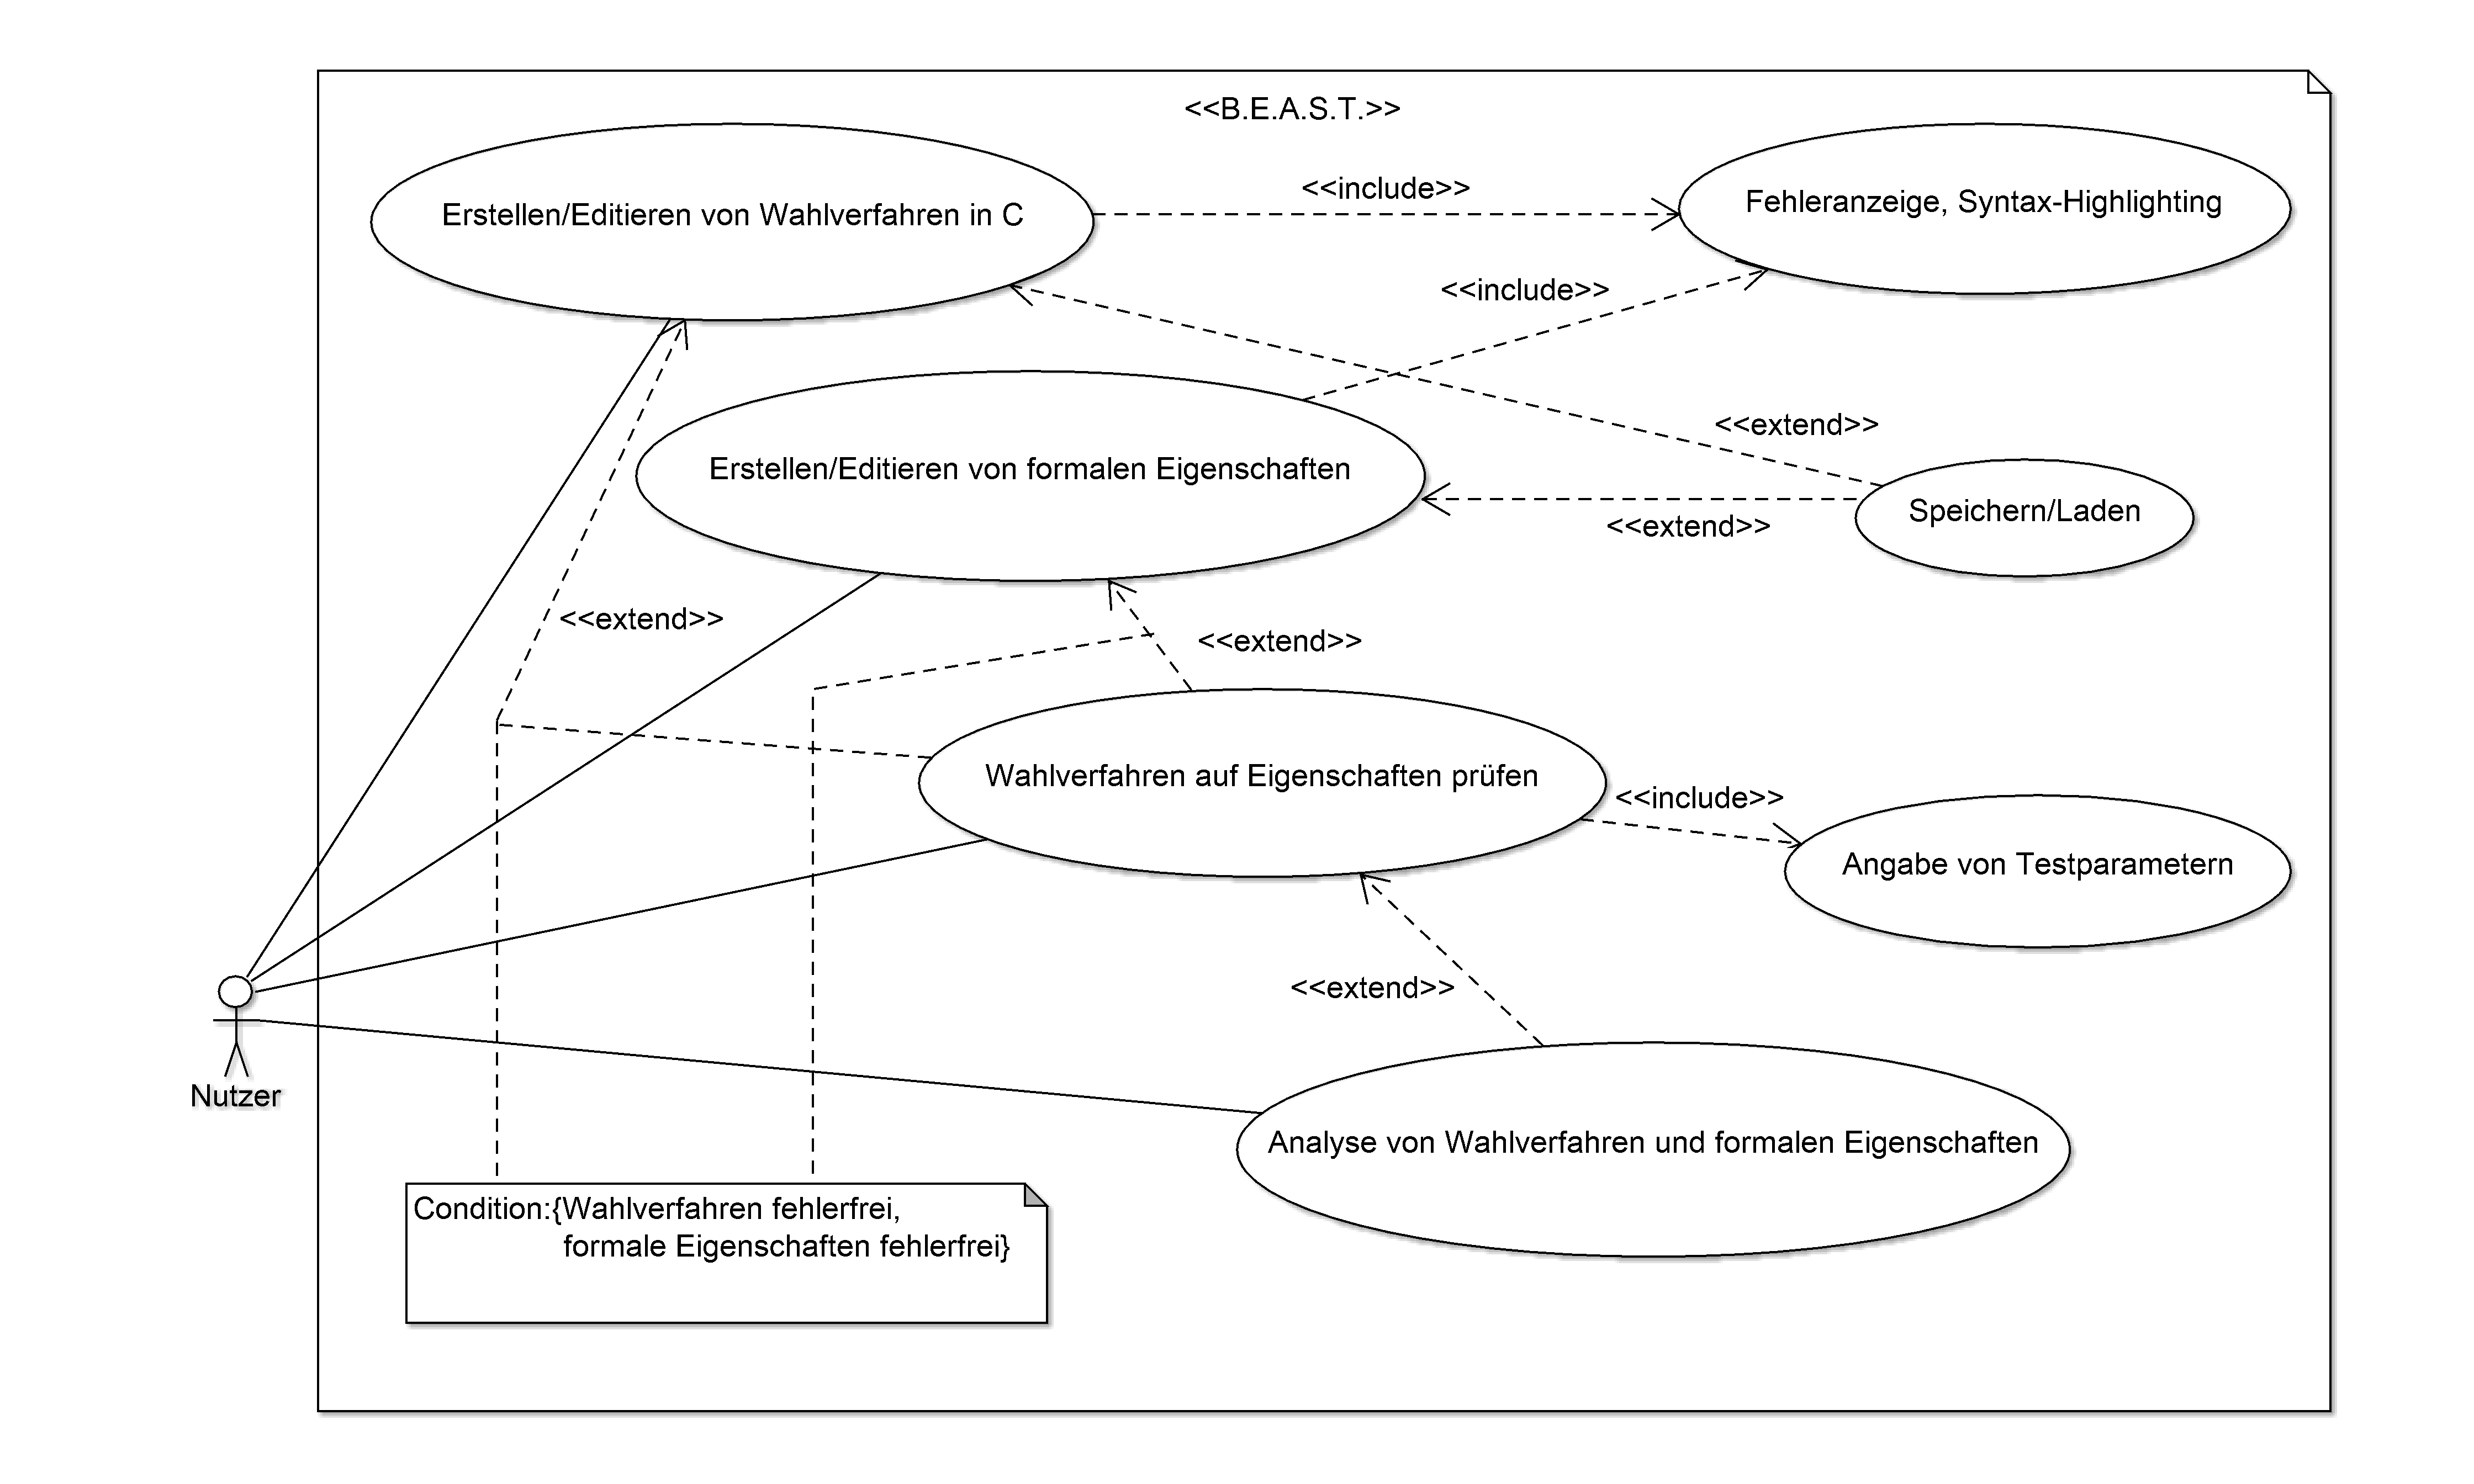
\includegraphics[scale=0.12]{UseCaseDiagram.png}
\caption{Anwendungsfalldiagramm von B.E.A.S.T.}
\label{Packet-scetch}
\end{figure}

Der Nutzer (Entwickler, Wahlforscher, Prüfstelle..) kann Wahlverfahren und formale Eigenschaften in den jeweiligen Editoren des Tools entwickeln bzw. editieren.
Beide Editoren verfügen über Optionen zum Laden und Speichern, sowie dem Anzeigen von Fehlern und Syntax-Highlighting.\\
Es kann geprüft werden ob das Wahlverfahren die formalen Eigenschaften erfüllt. Voraussetzung dafür sind ein fehlerfreies Wahlverfahren und fehlerfreie formale Eigenschaften. Vor dem Prüfen kann man Testparameter angeben (Anzahl von Kandidaten, Wählern, Sitzen und einem Timeout, dass dem Prüfen eine zeitliche Obergrenze gibt).\\
Nach dem Prüfen wird für jede Eigenschaft angezeigt ob sie vom Wahlverfahren erfüllt wird oder nicht. Bei Abbruch des Prüfens wegen erreichtem Timeout-Parameter werden natürlich nur die angezeigt die auch geprüft wurden. Werden formale Eigenschaften als nicht erfüllt erkannt, werden Gegenbeispiele angezeigt die die Nichterfüllbarkeit beweisen. Anhand dieser Informationen kann der Nutzer dann das Wahlverfahren und die Eigenschaften analysieren und falls nötig modifizieren.

\section{High-Level-Beschreibung der Architektur}	
Es folgt eine skizzenhafte Beschreibung der High-Level-Architektur des Softwaresystems. 

\begin{figure}[H]
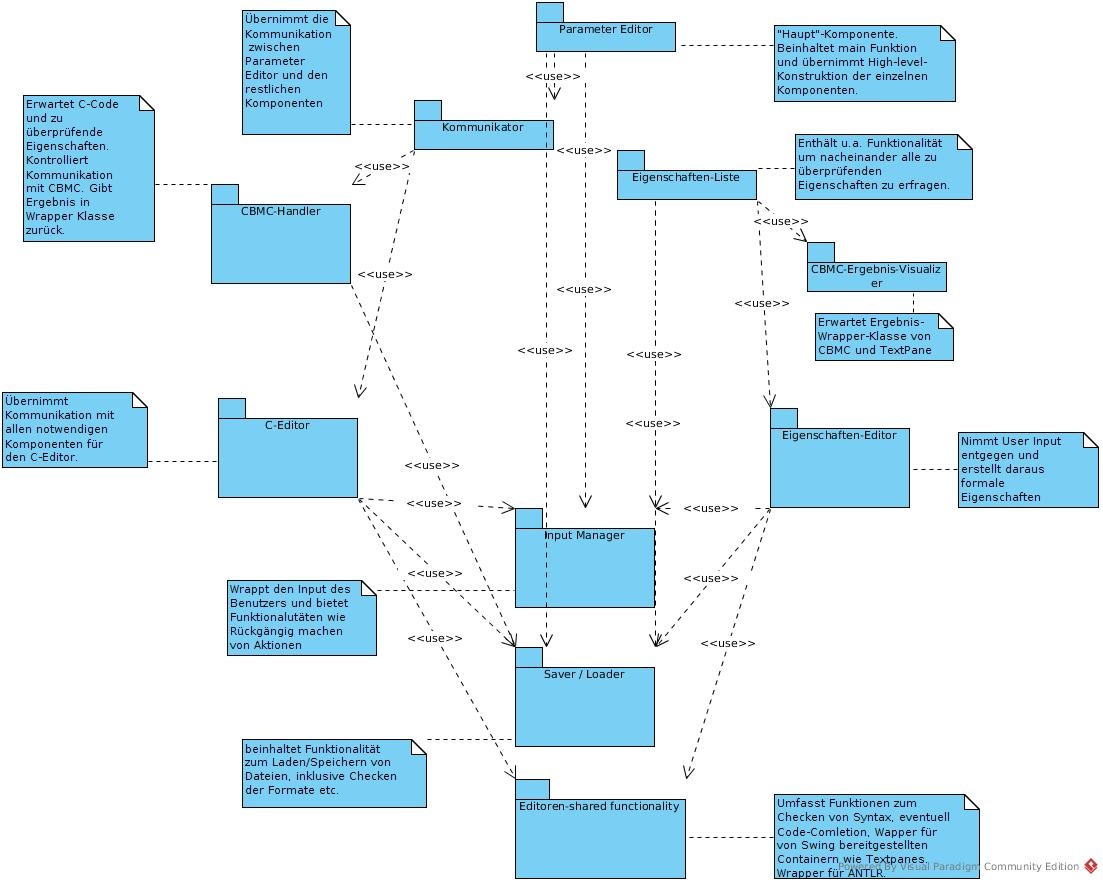
\includegraphics[scale=0.4]{architecture_first_scetch.jpg}
\caption{Skizzenhfte Beschreibung der Packete und ihrer Abhängigkeiten}
\label{Packet-scetch}
\end{figure}

\ref{Packet-scetch} zeigt einen ersten Entwurf der Packete und ihrer Abhängigkeiten untereinander. Diese einzelnen Packete sollen ähnliche Funktionalität bündeln. Zum momentanen Zeitpunkt liegen nur grobe Schätzungen vor wie aufwendig die implementierung der verschiedenen Funktionalitäten sein wird. Daher ist es möglich, dass manche Packete im Verlauf des Entwurfs als Klassen realisiert werden. Andernseits ist es auch möglich, dass weitere Packete hinzu kommen. Abhängigkeiten zu Java-Bibliotheken wie zum Beispiel Swing sind nicht dargestellt.

Ziel ist, möglichst  viel gemeinsame Funktionalität zu kapseln und wiederzuverwerten. Beispielsweiße haben C- und Eigenschaften-Editor viele analoge Aufgaben. Beide müssen Text darstellen und es dem Benutzer erlauben, diesen zu bearbeiten. Beide müssen eingegebenen Code auf syntaktische Fehler untersuchen und die Ergebisse dieser Untersuchung dem Benutzer signalisieren. Unterschiede wird es geben in den Regeln der einzuhaltenden Syntax sowie der \ac{GUI}. Daher wird diese Funktionalität gekapselt in einem eigenen Packet. 

Diese Kapselung setzt voraus, dass die verschiedenen Komponenten mit den korrekten Abhängigkeiten konstruiert werden. Funktionalität hierzu befindet sich in dem Dependency-Manager. Dieser stellt eine Schnittstelle da über welche man Instanzen der benötigten Komponenten beziehen kann. In dem Diagram werden dennoch die konkreten "benutzen" Beziehungen visualisiert. In dem konkreten Entwurf werden diese jedoch über den Dependency Manager geregelt. 

Das Kommunikator-Packet übernimmt die Kommunikation zwischen dem Parameter-Editor und den Komponenten. So wird es unter anderem der CBMC-Schnittstelle die korrekten Daten zukommen lassen und deren Ergebnisse an die Eigenschaften-Liste weiterleiten.

Alle Haupt-Komponenten müssen Dateien speichern und laden können. Ebenso müssen alle Haupt-Komponenten geladene Dateien auf korrektes Format hin überprüfen und das Ergebnis dieser Überprüfung mit dem Benutzer kommunizieren. Das mit Laden/Speichern beschriftete Packet wird Funktionalität zu diesem Zweck bereitstellen. 

Die CBMC-Schnittstelle erwartet die Beschreibung des Wahlverfahrens sowie die zu überprüfenden Eigenschaften (jeweils in Wrapper-Klassen). Sie erzeugt den Input für CBMC, ruft CBMC mit diesem Input auf und gibt das Ergebnis (in einer Wrapper-Klasse) zurück.

Diese Wrapper-Klassen erleichtern den Umgang mit den enthaltenen Daten. Die Wrapper-Klasse für CBMC-Ergebnisse wird Funktionen zur Abfrage der Wahleingaben und Wahlergebnisse bereitstellen. Die Wrapper-Klassen für Eigenschaften und C-Code werden es erleichtern, den für CBMC notwendigen Code zu generieren. Zusätzlich erleichtern sie eine Trennung der internen (Model) und externen (View) Darstellung der Daten. So kann die Visualisierung der CBMC-Ergebnisse von einer weiteren Klasse übernommen werden. Diese erwartet lediglich die Ergebnis-Wrapper-Klasse sowie eine Swing-Komponente auf welcher das Ergebnis darzustellen ist. Allgemein sorgt diese zusätliche  Abstraktion für eine flexible Architektur. Sollte das Program in Zukunft um weitere Programmiersprachen oder einen graphischen Editor zur Beschreibung von Wahlverfahren erweitert werden, so muss lediglich die entsprechende Wrapper-Klasse korrekt erzeugt werden.

Alle Editoren benötigen Funktionalität zum Wiederholen sowie Rückgängig machen von Aktionen. Dazu müssen Eingaben des Benutzers entsprechend gekapselt werden. Funktionaliät hierzu befindet sich im Input-Packet.

Sämtliche Resourcen wie Strings und durch den Benutzer konfigurierbare Eigenschaften wie der verwendete Font werden über den Resource Manager bereitgestellt. Dieser kann die vom Benutzer gegebenen Einstellungen auch speichern und laden.

\chapter{GUI}
Die hier vorgestellte \ac{GUI} erfüllt alle Muss-, Soll- und Kann-Kriterien. Das endgültige Produkt kann daher davon abweichen. Im Folgenden wird jedes mal darauf hingewiesen, falls es sich bei einem Feature um ein Kann-Kriterium handelt.
Die \ac{GUI} besteht aus 4 verschiedenen Fenstern: 
\begin{itemize}
\item Ein Editor für C-Code, in welchem die Wahlverfahren editiert werden können
\item Eine Liste, in welcher alle für dieses Wahlverfahren zu überprüfenden Eigenschaften angezeigt werden
\item Ein Editor in welchem Eigenschaften editiert werden können
\item Das Hauptfenster, dessen Schließen ein Beenden des kompletten Tools nach sich zieht. Darin können Parameter für Überprüfungen eingestellt und Überprüfungen gestartet bzw. beendet werden
\end{itemize}
Jedes dieser Elemente verfügt auch über weitere Eigenschaften, die im Folgenden beschrieben werden.

\section{C-Editor}
Der C-Editor verfügt über dieselbe Funktionalität, welche andere Texteditoren wie zum Beispiel Notepad aufweisen. Ziel ist es, das Eingeben von Funktionen, welche ein Wahlverfahren implementiert, zu ermöglichen. Dazu bietet er die Möglichkeit, C-Code zu schreiben und zu bearbeiten. Ein angemessener Funktionskörper, welcher die auswählbare Art der Wahl, repräsentiert, wird dabei automatisch generiert (siehe \ref{Editor-mit-text}). Es wird nicht möglich sein, diese Funktion zu editieren. Während des Eingebens des Codes wird dieser automatisch analysiert, um Schlüsselwörter sowie syntaktische Fehler zu markieren. 
Der C-Editor teilt sich in vier Untereinheiten auf: Der Menüstreifen, die Tool-Leiste, das Textfeld und das Fehlerfeld. Der Menü-Streifen ist unterteilt in Datei, Bearbeiten, Editor (Kann) und Code. Bilder aller geöffneten Untermenüs befinden sich im Anhang. Sie beinhalten folgende Funktionalität:

\begin{table}[H]
\begin{tabular}{|p{3cm}|p{12cm}|}
Menüpunkt & Bedeutung \\
\hline
Neu & öffnet ein neues Dokument, wobei die Art der Wahl vom User angegeben wird \\
Speichern & speichert das Dokument unter bereits gegebenem Namen \\
Speichern unter & Speichert das Dokument unter neuem Namen an neuem Ort, beide durch User angegeben \\
Öffnen & Öffnet neues Dokument des richtigen Formats
\end{tabular}
\label{Datei-Menüpunkte}
\caption{Unterpunkte des Datei-Menüs}
\end{table}

\begin{table}[H]
\begin{tabular}{|p{3cm}|p{12cm}|}
Menüpunkt & Bedeutung \\
\hline
Rückgängig & Falls möglich: Macht die letzte ausgeführte Aktion Rückgängig \\
Wiederholen & Wiederholt die zuletzt Rückgängig gemachte Aktion \\
Kopieren & Fügt markierten Text in die Zwischenablage ein \\
Ausschneiden & Fügt markierten Text in die Zwischenablage ein und entfernt ihn aus dem Textfeld \\
Einfügen & Fügt Text aus der Zwischenablage an der Stelle des Cursors ein \\
Wahlart ändern & Ändert den Funktionskörper zu dem der vom User ausgewählten Art
\end{tabular}
\label{Bearbeiten-Menüpunkte}
\caption{Unterpunkte des Bearbeiten-Menüs}
\end{table}

\begin{table}[H]
\begin{tabular}{|p{3cm}|p{12cm}|}
Menüpunkt & Bedeutung \\
\hline
Einstellungen & Öffnet den Einstellungen-Dialog. Dies ist Teil der Kann-Kriterien. Falls implementiert, wird es Möglichkeiten zur Einstellung des Fonts und Syntax-Highlighting geben.
\end{tabular}
\label{Editor-Menüpunkte}
\caption{Unterpunkte des Editor-Menüs}
\end{table}

\begin{table}[H]
\begin{tabular}{|p{3cm}|p{12cm}|}
Menüpunkt & Bedeutung \\
\hline
Statische Analyse & Startet eine statische Analyse des Codes, welche ihn auf von Lexer oder Parser erkennbare Fehler untersucht. Gefundene Fehler werden in dem Fehlerfeld angezeigt. Zusätzliches Kann-Kriterium: Die Zeile, in welcher der Fehler ist, wird zusätzlich durch einen roten Punkt markiert (siehe \ref{Editor-mit-Fehler-nach-statischer-analyse}
\end{tabular}
\label{Editor-Menüpunkte}
\caption{Unterpunkte des Code-Menüs}
\end{table}

\begin{figure}[H]
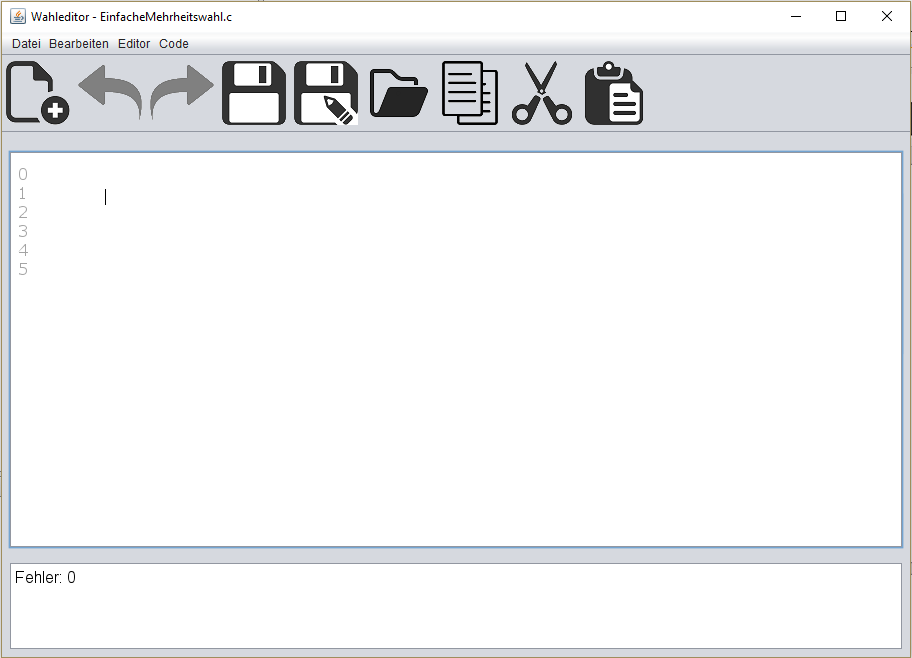
\includegraphics[scale=0.5]{Editor-ohne-text.png}
\caption{Der C Editor ohne Code. Direkt unter dem Menü-Streifen befindet sich der Tool-Streifen}
\label{C-Editor-Tool-Streifen}
\end{figure}

Über den Tool-Streifen (siehe \ref{C-Editor-Tool-Streifen}) lassen sich einige dieser Aktionen ohne Öffnen eines Menüs ausführen. Von Links nach Rechts: Neu, Rückgängig, Wiederholen, Speichern, Speichern unter, Öffnen, Kopieren, Ausschneiden, Einfügen. Aktivieren der Aktion "'Neu"' öffnet einen Dialog, welcher vim Nutzer die Eingabe folgender Eigenschaften erwartet: Speicherort, Name und Kategorie des Wahlverfahrens.

\begin{figure}[H]
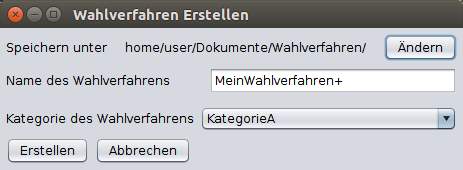
\includegraphics[scale=0.5]{Wahlverfahren-Erstellen.png}
\caption{Der Dialog welcher dem User das Erstellen neuer Wahlverfahren ermöglicht}
\label{C-Editor-Tool-Streifen}
\end{figure}

Bei erfolgreicher Eingabe wird eine neue Datei geöffnet, welche der Nutzer editieren kann. Die Kategorie des Wahlverfahrens wird durch die Funktionssignatur der Wahlfunktion (\texttt{voting}) dargestellt, welche nicht vom Nutzer verändert werden kann. 

\begin{figure}[H]
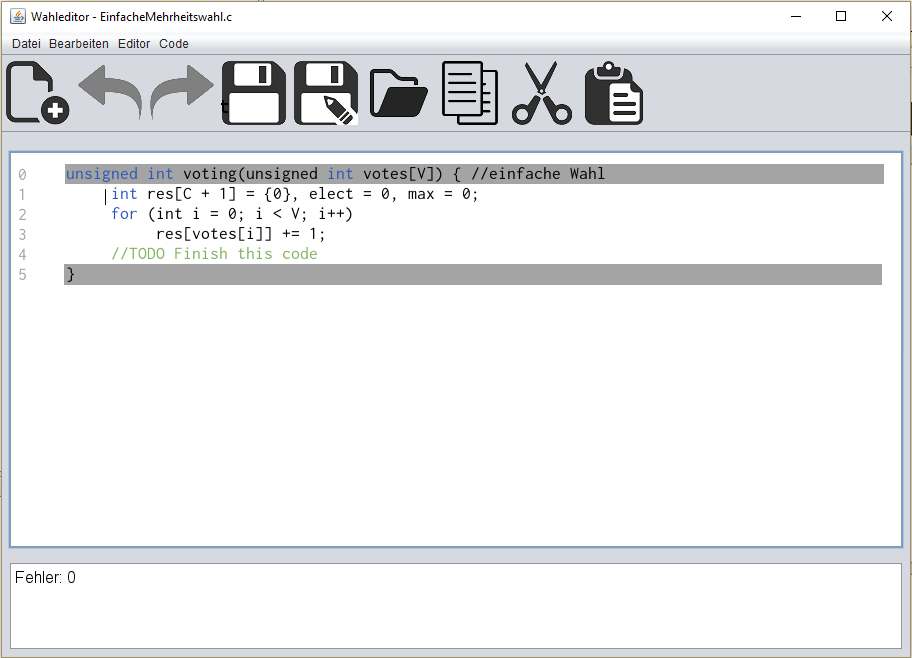
\includegraphics[scale=0.4]{Editor-mit-text.png}
\caption{Der C Editor mit Code und Anzeige der Wahlart}
\label{Editor-mit-text}
\end{figure}

In \ref{Editor-mit-text} sieht man den Editor nach Eingabe diverser Elemente der C-Sprache. Anzeige der Zeilennummern ist Soll-Kriterium, Möglichkeit diese Funktion zu deaktivieren Kann-Kriterium. Die grauen Balken zeigen an, dass man den vorgegebenen Funktionskörper nicht editieren kann. Der Kommentar rechts der Funktionsdefinition gibt die Kategorie des Wahlverfahrens an.

\begin{figure}[H]
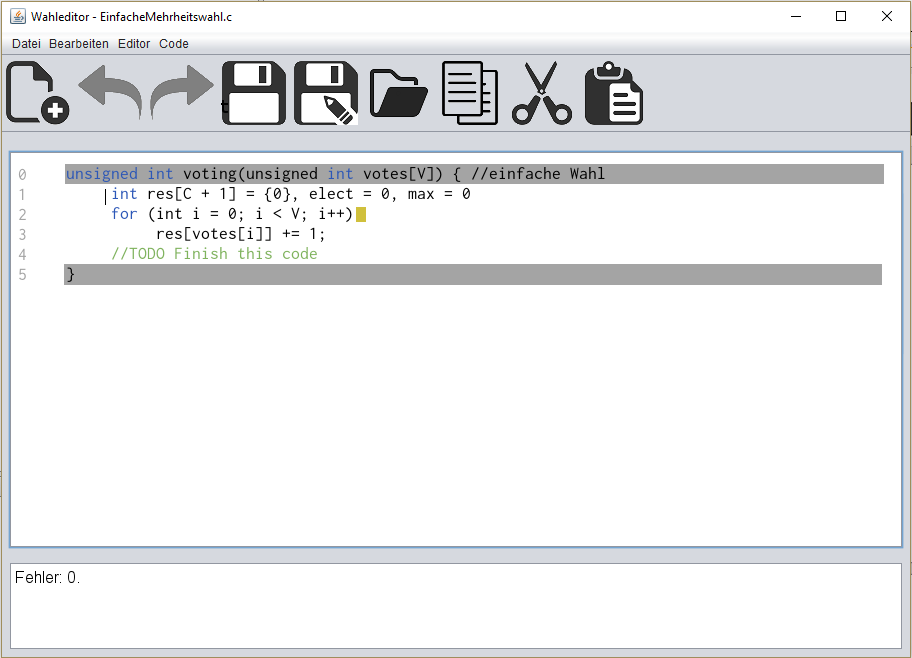
\includegraphics[scale=0.4]{Editor-mit-Fehler-ohne-hover.png}
\caption{Fehleranzeige bei syntaktischem Fehler ohne Maus-Hover (Kann-Kriterium)}
\label{Editor-mit-Fehler-ohne-hover}
\end{figure}

\begin{figure}[H]
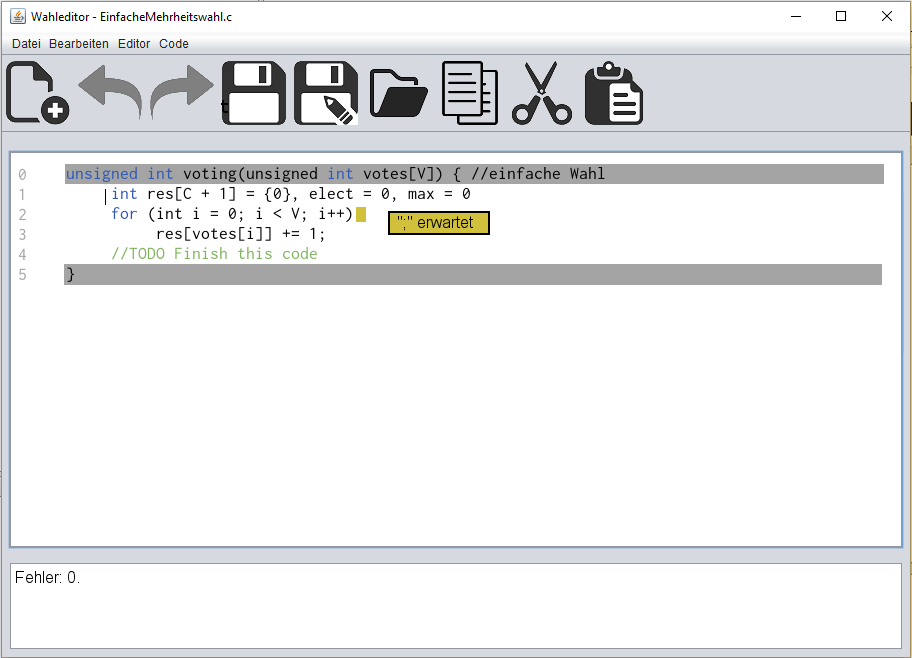
\includegraphics[scale=0.4]{Editor-mit-Fehler-mit-hover.png}
\caption{Fehleranzeige bei syntaktischem Fehler mit Maus-Hover (Kann-Kriterium)}
\label{Editor-mit-Fehler-mit-hover}
\end{figure}

In \ref{Editor-mit-Fehler-ohne-hover} sieht man, wie der gefundene syntaktische Fehler während des Editieren des Codes angezeigt wird. Dies ist ein Kann-Kriterium. Sobald man mit der Maus über die markierte Stelle geht, wird in einem neuen Fenster nahe der Maus eine Beschreibung des Fehlers angezeigt. Dies ist ebenfalls Kann-Kriterium (siehe \ref{Editor-mit-Fehler-mit-hover}).

\begin{figure}[H]
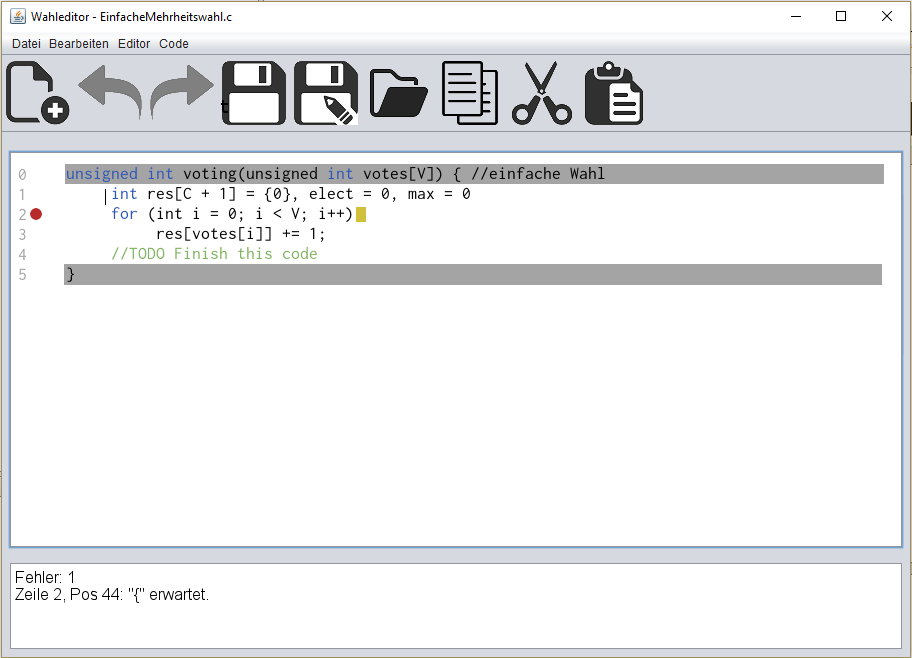
\includegraphics[scale=0.4]{Editor-mit-Fehler-nach-statischer-analyse.png}
\caption{Fehleranzeige nach statischer Analyse}
\label{Editor-mit-Fehler-nach-statischer-analyse}
\end{figure}

\ref{Editor-mit-Fehler-nach-statischer-analyse} Zeigt die Anzeige der Fehler nach ausführend einer statischen Code Analyse. Markierung der Zeile ist Kann-Kriterium.

\section{Eigenschaften-Liste}
Die GUI trennt das Editieren der zu überprüfenden Eigenschaften (in eigens zu diesem Zweck erstellter Syntax, siehe \ref{Sprache-für-formale-Eigenschaften}) und das Zuordnen dieser Eigenschaften zu Wahlverfahren. Dadurch können diese Eigenschaften einzeln abgespeichert und flexibel wiederverwertet und kombiniert werden. Das Zuordnen der Eigenschaften zu Wahlverfahren geschieht in der Eigenschaften-Liste. Darin werden die einzelnen Eigenschaften namentlich aufgelistet (siehe \ref{Eigenschaften-Liste-vor}). 

\begin{figure}[H]
\begin{minipage}{.5\textwidth}
  \centering
  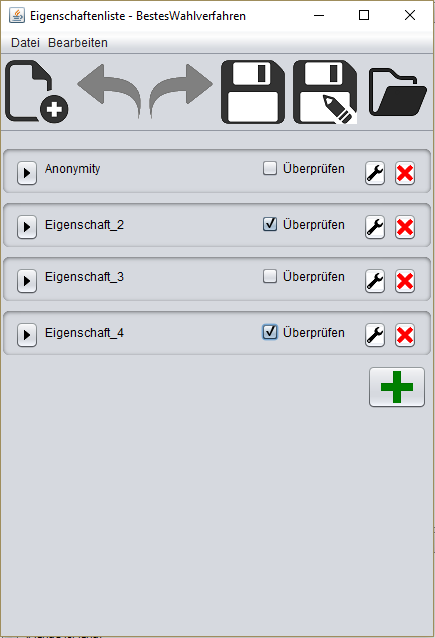
\includegraphics[scale=0.5]{Eigenschaften-Liste.png}
  \caption{Eigenschaften-Liste vor einer Überprüfung}
  \label{Eigenschaften-Liste-vor}
\end{minipage}
\begin{minipage}{.5\textwidth}
  \centering
  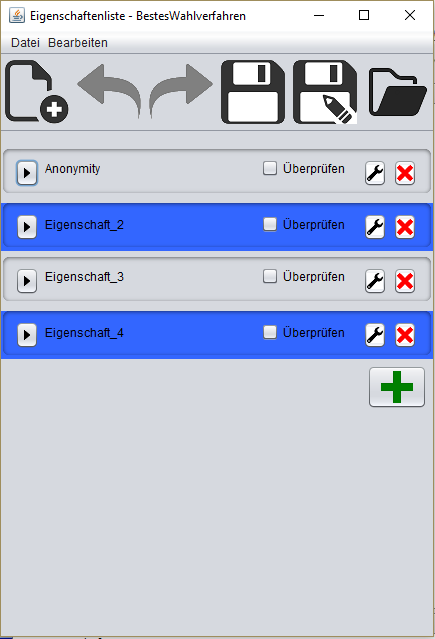
\includegraphics[scale=0.5]{Eigenschaften-Liste-waehrend-testen.png}
  \caption{Eigenschaften-Liste während einer Überprüfung}
  \label{fig:sub2}
\end{minipage}
\end{figure}

Im Folgenden werden die einzelnen \ac{GUI}-Bestandteile und der Funktionalität erläutert.

\begin{table}[H]
\begin{tabular}{|p{3cm}|p{12cm}|}
Menüpunkt & Bedeutung \\
\hline
Neu & Startet eine neue Liste \\
Speichern & Speichert die Liste \\
Speichern unter & Speichert die Liste unter neuem Namen an neuem Ort \\
Öffnen & öffnet Liste (Ort von User angegeben)
\end{tabular}
\label{Eigenschaftenliste-Datei-Menüpunkte}
\caption{Unterpunkte des Datei-Menüs}
\end{table}

\begin{table}[H]
\begin{tabular}{|p{3cm}|p{12cm}|}
Menüpunkt & Bedeutung \\
\hline
Rückgängig & Falls möglich: Macht die letzte ausgeführte Aktion Rückgängig \\
Wiederholen & Wiederholt die zuletzt Rückgängig gemachte Aktion 
\end{tabular}
\label{Eigenschaftenliste-Bearbeiten-Menüpunkte}
\caption{Unterpunkte des Bearbeiten-Menüs}
\end{table}

Der Tool-Streifen hat exakt den selben Zweck wie der des Code-Editors, ohne die Funktionen Kopieren, Ausschneiden und Einfügen.

\begin{figure}[H]
\begin{minipage}{.5\textwidth}
  \centering
  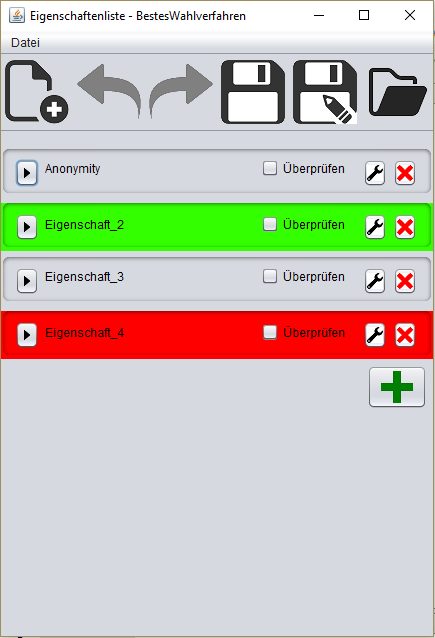
\includegraphics[scale=0.5]{nach-testen.png}
  \caption{Liste nach Überprüfung}
  \label{fig:sub1}
\end{minipage}
\begin{minipage}{.5\textwidth}
  \centering
  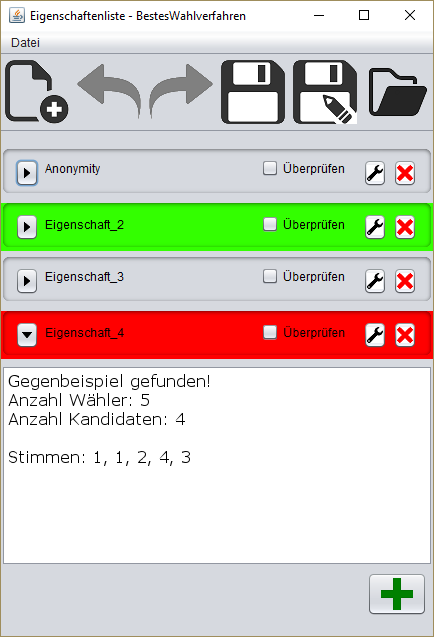
\includegraphics[scale=0.5]{gegenbeispiel.png}
  \caption{Anzeige des Gegenbeispiels}
  \label{fig:sub2}
\end{minipage}
\end{figure}

Es folgt eine Beschreibung der Icons, welche in den Listenelementen zu sehen sind.

\begin{table}[H]
\begin{tabular}{|p{3cm}|p{12cm}|}
Icon & Bedeutung \\
\hline
Pfeil nach rechts & Falls Gegenbeispiel gefunden: Durch Klicken öffnet sich unter dem Listenelement ein Textfeld in welchen das Gegenbeispiel dargestellt wird \\
Checkbox & Nur falls aktiviert, wird das Wahlverfahren auf die Eigenschaft getestet \\
Maulschlüssel & Öffnet den Eigenschaften-Editor für die Eigenschaft\\
Rotes Kreuz & Entfernt die Eigenschaft aus der Liste \\
Gründes Plus & Fügt neue, leere Eigenschaft oder bereits gespeicherte Eigenschaft der Liste hinzu
\end{tabular}
\label{Eigenschaftenliste-Bearbeiten-Menüpunkte}
\caption{Icons der Eigenschaften-Liste}
\end{table}

\section{Eigenschaften-Editor}

\begin{figure}[H]
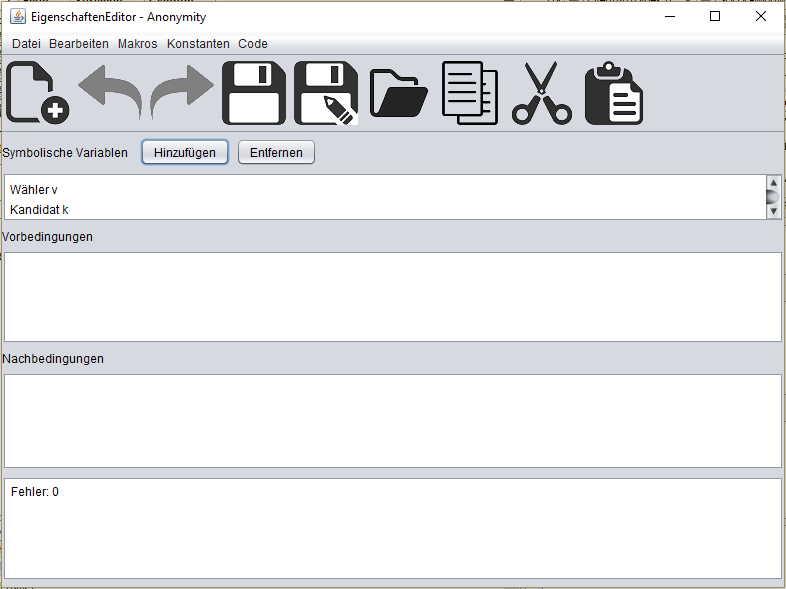
\includegraphics[scale=0.5]{raw-ohne-code.png}
\caption{Eigenschaften-Editor ohne Code mit symbolischen Variablen}
\label{Eigenschaften-Editor-ohne-code}
\end{figure}

Der Eigenschaften-Editor hat den Zweck, das Bearbeiten der zu überprüfenden Eigenschaften zu ermöglichen. Eigenschaften werden aufgeteilt in Vor- und Nachbedingungen. Möglich ist die Verwendung sowohl von Quantoren in der Form von Makros als auch symbolischer Variablen. 

Die Untermenüs Datei, Bearbeiten und Code sowie der Tool-Streifen sind analog zu denen des C-Editors. Hinzu kommen jedoch Konstanten und Makros. Bereitgestellte Konstanten sind: 

\begin{itemize}
\item Die Anzahl der Wähler (V)
\item Die Anzahl der Kandidaten (C)
\item Die Anzahl vorhandener Sitze (S)
\end{itemize}

Bereitgestellte Makros sind:

\begin{itemize}
\item \verb!FOR_ALL_VOTERS()!
\item \verb!FOR_ALL_CANDIDATES()!
\item \verb!FOR_ALL_SEATS()!
\item \verb!EXISTS_ONE_VOTER()!
\item \verb!EXISTS_ONE_CANDIDATES()!
\item \verb!EXISTS_ONE_SEAT()!
\item \verb!SUM_VOTES_FOR_CANDIDATE()!
\end{itemize}

Jedes dieser Makros bis auf das Letzte nimmt eine bisher ungenutzte Variable als Argument. Diese kann im darauf Folgenden boolschen Ausdruck verwendet werden (siehe \ref{Eigenschaften-Editor-Anonymität}). Das Letzte Makro nimmt eine bereits definierte symbolische Variable vom Typ Kandidaten und gibt berechnet die Anzahl Stimmen für diesen Kandidaten.

\begin{figure}[H]
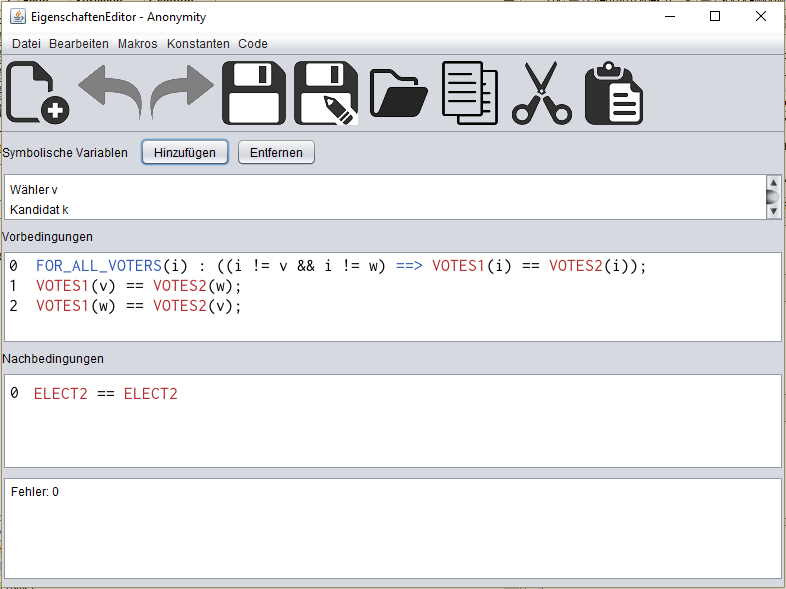
\includegraphics[scale=0.5]{Editor-vor-und-nachbedingungen-syntax-highlighting.png}
\caption{Eigenschaften-Editor mit Beispielhafter Eigenschaft Anonymität und beispielhaft dargestelltem Syntax-Highlighting (Kann-Kriterium)}
\label{Eigenschaften-Editor-Anonymität}
\end{figure}

Wie man zusätzlich sehen kann, sind auch Implikationen (\verb!==>!) möglich. Auch das logische und (\verb!&&!), oder (\verb!||!) und die Äquivalenz (\verb!<==>!) werden zur Verfügung stehen. Die Anzeige erkannter Fehler wird analog zum C-Editor geschehen.

\section{Parameter Editor}

Der Parameter Editor stellt das Hauptfenster der Anwendung dar. Es erlaubt das Einstellen und Starten der Tests. Hier lassen sich auch komplette Projekte Speichern - Code, Eigenschaften und Parameter gebündelt.

\begin{figure}[H]
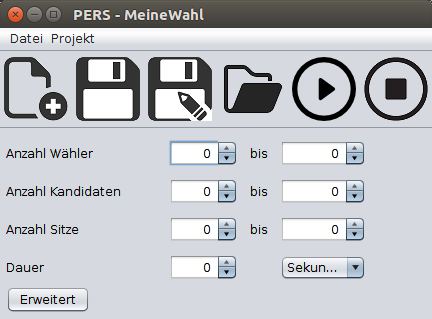
\includegraphics[scale=0.6]{Parameter-Editor.png}
\caption{Der Parameter Editor. PERS steht für Professional Election Rigging System}
\label{Parameter-editor}
\end{figure}

Der Menüpunkt Datei ist analog zu dem des C Editors. Der Menüpunkt Projekt wird im Folgenden erläutert. 

\begin{table}[H]
\begin{tabular}{|p{5cm}|p{10cm}|}
Menüpunkt & Bedeutung \\
\hline
Teste Eigenschaften & Startet Tests mit den angegebenen Parametern \\
Stop Test & Unterbricht momentan laufenden Test
\end{tabular}
\label{Parameter-Projekt-Menü}
\caption{Parameter Editor Projekt Menüpunkte}
\end{table}

Der Pfeil und das Stopp-Zeichen des Tool-Streifens haben ebenfalls die Wirkungen Teste Eigenschaften und Stop Test. Als Mögliche Zeitangaben stehen Sekunden, Minuten, Stunden und Tage zur Verfügung. 

\begin{figure}[H]
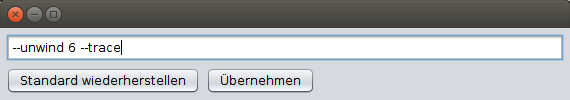
\includegraphics[scale=0.6]{CBMC-Args-Editor.png}
\caption{Das Fenster, welches dem \gls{Benutzer} erlaubt die an CBMC gereichten Argumente zu editieren}
\label{Argumente-editor}
\end{figure}

Klickt der \gls{Benutzer} auf Erweitert, so öffnet sich Dialog \ref{Argumente-editor}. Darin kann der \gls{Benutzer} direkt die an \ac{CBMC} gereichten Argumente editieren. Vom \gls{Benutzer} gegebene Argumente unterliegen keiner Überprüfung durch das Program und führen daher zu undefiniertem Verhalten. 

\chapter{Zeit- und Resourcenplanung}

Für den Rest des Projektes veranschlagen wir 1500 Mannstunden. Die Verteilung
der Stunden sieht wie folgt aus.

\section{Zeitplan}

\begin{table}[H]
\centering
  \begin{tabular}{|p{3cm}|P{2cm}|P{2cm}|}
    Phase & Zeitraum & Studen \\ \hline
    Entwurf & 05.12.16 - 16.01.17 & 480 Mannstunden \\ \hline
    Implementierung & 18.01.17 - 13.02.17 & 560 Mannstunden \\ \hline
    Qualitätssicherung & 01.03.1 - 20.03.17 & 480 Mannstunden \\
  \end{tabular}
  \newline\newline
  \caption{Zeiträume und Arbeitsanteile}\label{tab1}
\end{table}


\section{Unteraufteilung der Phase}
Nun unterteilen wir die einzelnen Phasen in ihre Unterbestandteile,
zusammen mit den Veranschlagungen für den veranschlagten Anteil am Gesamtaufwand
der Phase.

\subsection{Entwurfsphase}

\begin{table}[H]
\centering
  \begin{tabular}{|p{3cm}|P{2cm}|P{2cm}|}
    Sub-Phase & Anteil \\ \hline
    GUI & 35\%\\ \hline
    C-Code Analyse & 30\%\\ \hline
    Dateiverwaltung & 10\%\\ \hline
    Rest & 25\%\\
  \end{tabular}
  \newline\newline
  \caption{Unteraufteilung der Entwurfsphase}\label{entw}
\end{table}

\subsection{Implementierungsphase}

\begin{table}[H]
\centering
  \begin{tabular}{|p{3cm}|P{2cm}|P{2cm}|}
    Sub-Phase & Anteil \\ \hline
    GUI & 35\%\\ \hline
    C-Code Analyse & 30\% \\ \hline
    Dateiverwaltung & 10\% \\ \hline
    Rest & 25\%  \\
  \end{tabular}
  \newline\newline
  \caption{Unteraufteilung der Implementierungsphase}\label{impl}
\end{table} 

\subsection{Qualitätssicherung}
\begin{table}[H]
\centering
  \begin{tabular}{|p{3cm}|P{2cm}|P{2cm}|}
    Sub-Phase & Anteil \\ \hline
    Test der GUI & 25\% \\ \hline
    Testfälle  für die Codeanalyse & 25\% \\ \hline
    Testfälle für CBMC & 15\% \\ \hline
    Test des Dateisystems & 10\% \\ \hline
    Rest & 25\%  \\
  \end{tabular}
  \newline\newline
  \caption{Unteraufteilung der Entwurfsphase}\label{qs}
\end{table}


\chapter{Phasenverantwortliche}
\section{Pflichtenheft} Justin Hecht
\section{Entwurf} Holger Klein 
\section{Implementierung} Niels Hanselmann, Nikolai Schnell
\section{Qualitätssicherung} Lukas Stapelbroek
\section{Abschlusspräsentation} Jonas Wohnig


\chapter{Qualitätsanforderungen}

\begin{table}[H]
  \centering
  \begin{tabular}{|P{3cm}|P{2cm}|P{2cm}|P{2cm}|P{2cm}|}
    Name & sehr gut & gut & normal & nicht relevant\\ \hline
    Fehlertoleranz & x &  &  &  \\ \hline
    Sicherheit & x &  &  &  \\ \hline
    Bedienbarkeit &  &  &  & x \\ \hline
  	Zeitverhalten Editor &  & x &  &  \\ \hline
  	Zeitverhalten Analyse &  &  &  & x \\ \hline
  	Erlernbarkeit &  & x &  &  \\ \hline 
    Modifizierbarkeit & x &  &  &  \\
  \end{tabular}
  \newline\newline
  \caption{Qualitätsanforderungen}\label{qa}
\end{table}


\printglossaries
 

 
\end{document}
